%----------------------------------------------------------------------
% HAUPTDATEI
% Enthlt die Verknpfungen aller Dateien zur gesamten Diplomarbeit
%----------------------------------------------------------------------

%----------------------------------------------------------------------
% HEADER
% Einstellungen, Makros etc.
%----------------------------------------------------------------------
\documentclass[12pt,a4paper,twoside,scrartcl,report]{thesis}
\NeedsTeXFormat{LaTeX2e}[1994/06/01]

% Verwendete Pakete
\usepackage{ae}
\usepackage{times}
\usepackage[ngerman]{babel}					% Deutsche Besonderheiten (neue Rechtschreibung)
\usepackage[utf8]{inputenc}				% Latin-1 (z.B. ß)
\usepackage[T1]{fontenc}						% T1-Schriften verwenden (statt CM)
\usepackage{textcomp}								% Zusätzliche Textsymbole von T1
\usepackage{makeidx}								% Index
\usepackage{fancyhdr}								% Definition von Kopf-/Fußzeilen
\usepackage{psboxit}
\usepackage{float}									% Gleitumgebungen
\usepackage{setspace}
\usepackage{doc}										% Für's BibTeX-Logo (Siehe vorlage.tex)
\usepackage{changebar}
\usepackage{listings}								% Formatierungen für Quellcode
%\usepackage{color}
\usepackage{multirow}
\usepackage{longtable}							% Tabellen über mehrere Seiten
\usepackage{multicol}								% Mehrspaltiger Satz
\usepackage[german]{varioref}				% Variable Referenzen
\usepackage{lscape}									% Querformat
\usepackage{footnpag}								% Fußnoten: Nummerierung auf jeder Seite bei 1 beginnen
\usepackage[normalem]{ulem}					% Unterstreichung
\usepackage{xspace}
\usepackage[bottom,hang,marginal]{footmisc}
\usepackage{amsmath}
\usepackage[bf,SL,BF]{subfigure}
\usepackage{gastex}
\usepackage{array}
\usepackage{eurosym}
\usepackage{ragged2e}
\usepackage{url}

% Die Algorithmus-Umgebung für Pseudocode
\usepackage{algorithmic}
\usepackage{algorithm}
\numberwithin{algorithm}{chapter}
\renewcommand{\listalgorithmname}{Verzeichnis der Algorithmen} 
\renewcommand{\algorithmiccomment}[1]{// #1}
\floatname{algorithm}{Algorithmus}
\newcommand{\theHalgorithm}{\arabic{algorithm}}
%\setlength{\footnotemargin}{0pt}

% set font-style to computer modern sans-serif (cmss)
%\renewcommand{\sfdefault}{cmss}
%\renewcommand{\familydefault}{\sfdefault}

%----------------------------------------------------------------------
% Besondere Einstellungen für PDF-Ausgabe.
% Es wird eine Fallunterscheidung getroffen und entsprechende Pakete
% eingebunden und Einstellungen vorgenommen.

% PDF oder DVI? Es wird ein Flag gesetzt.

% PDF Einstellungen
\RequirePackage{ifpdf}
\ifpdf
  \usepackage{graphicx}
  \pdfcompresslevel=9
  \usepackage[
  		pdftex, 
  		colorlinks=true,
  		linkcolor=blue,
  		urlcolor=blue,
  		citecolor=blue,
  		plainpages=false,
  		pdfpagelabels,
  		bookmarksnumbered=true,
			pdftitle={Thema der Arbeit eintragen!},
			pdfauthor={Max Mustermann},
			pdfkeywords={Key, Words} ]{hyperref}
  % PDF-Seite bei LScape-rotate drehen
  \makeatletter
  \@ifundefined{pdfpageattr}
    {}{\g@addto@macro{\landscape}{\pdfpageattr{/Rotate 90}}}
  \makeatother
% DVI (oder andere Ausgabe) Einstellungen
\else
  \usepackage[dvips]{graphicx}		% Graphikunterstützung, auch JPG und PNG
\fi

% Erlaubt das Einbinden von JPGs in das Dokument (aus Paket [dvips]{graphicx}).
% Die JPGs werden zuvor nach EPS konvertiert. Die Größe (BoundingBox)ist in <datei>.bb
% festgelegt. Diese muß manuell durch ebb.exe erzeugt werden.
\DeclareGraphicsRule{.jpg}{eps}{.bb}{}

%-----------------------------------------------------------------------
% Seitenlayout festlegen
\voffset-1in
\hoffset-1in
\setlength{\oddsidemargin}{4cm}
\setlength{\evensidemargin}{2cm}
\topmargin15pt
\textwidth150mm
\textheight230mm
\footskip1.5cm
\headheight25pt

\pagestyle{fancyplain}

% Definition von Kopf- und Fußzeilen
\lhead[\fancyplain{}{\nouppercase{\sl\rightmark}}]{\fancyplain{}{\nouppercase{\sl\leftmark}}}
%\rhead[\fancyplain{}{\nouppercase{\sl\leftmark}}]{\fancyplain{}{\nouppercase{\sl\leftmark}}}
\rhead[\fancyplain{}{\nouppercase{\sl\leftmark}}]{\fancyplain{}{\nouppercase{\sl\rightmark}}}
%-----------------------------------------------------------------------
% Definitionen für Quellcodes/Listings
\lstloadlanguages{Java}
\lstset{
  language=[AspectJ]Java,						% Java with AspectJ-Dialect
	tabsize=4,												% Tabulatorbreite
	linewidth=\linewidth,							% Width of a line
	breaklines=true,									% Break long lines
	breakatwhitespace=true,						% Only break at whitespaces
	basicstyle=\scriptsize\ttfamily,	% Schriftart/-größe	
	numbers=left,											% Linenumbers left
	numberfirstline=false,						% Not: Always number 1. line
	numberstyle=\scriptsize,					% Größe der Zeilennummern
	stepnumber=1,											% Jede 2. Zeilennummer anzeigen
	numbersep=5pt,										% Abstand Nr - Quellcode
	showspaces=false,									% Spaces nicht anzeigen
	showtabs=false,										% Tabs nicht anzeigen
	showstringspaces=false,						% Don't show tabs in strings
	showlines=false,									% Leerzeilen am Sourceende weglassen
	extendedchars=true,								% ASCII-Zeichnen > 127 zulassen 
	identifierstyle=\bfseries,					% Identifier
	keywordstyle=\bfseries,						% Keywords
	commentstyle=\itshape,						% Style of comments
	stringstyle=\ttfamily,						% Strings (!= Keywords)
	flexiblecolumns=false,						% Use fixed width for fonts
	fontadjust=true,									% "Base width" nicht jede Zeile anpassen
	frame=trbl,												% Frame; trBL
	captionpos=b,											% Position of the caption
	aboveskip=25pt,										% Space between text and the top of the listing
}

%-----------------------------------------------------------------------
%VERZEICHNISSE 

\makeindex

% Namen für Quellcodes und Quellcode-Verzeichnis
\renewcommand\lstlistingname{\normalsize Quellcode}
\renewcommand\lstlistlistingname{Verzeichnis der Quellcodes}

% Layout für Literaturverzeichnis (BibTeX)
\bibliographystyle{alphadin}			% Alphab., Verfasser + Jahr (DIN 1502)

% Inhaltsverzeichnis
\setcounter{tocdepth}{3}
\setcounter{secnumdepth}{3}

\makeatother

%-----------------------------------------------------------------------
% Debug-Optionen - sollten fuer die Final Version gelöscht werden
\vrefwarning
\nochangebars

% Tabellen über Seitengrenzen zulassen
\setlongtables

% Absatztrennung durch Abstand - keine Einrückung
\setlength\parskip{\medskipamount}
\setlength\parindent{0pt}

% Abstand Text - Graphik (nur Mitten in Text)
\setlength{\intextsep}{25pt plus 3pt minus 2pt}
%-----------------------------------------------------------------------
% EIGENE KOMMANDOS
\PScommands
% \todo{<text>}: TODO-Hinweis
\newcommand{\todo}[1]{\psboxit{box .7 setgray fill}{\spbox{TODO: [#1]}}\bigskip}
% \comment{<text>}: Kommentar, nicht im Dokument sichtbar
\newcommand{\comment}[1]{}
% \markup{<test>}: Unterstrichener Text
\newcommand{\markup}[1]{\uline{#1}}
% \file{<text>}: Formatierung für Dateinamen
\newcommand{\file}[1]{{\sffamily #1}}
% \code{<text>}: Formatierung von "Code" (Klassenname, Methodennamen etc.) im Fließtext
\newcommand{\code}[1]{\mbox{\texttt{#1}}}
%-----------------------------------------------------------------------
% Spezielle TRENN-VORGABEN
\hyphenation{Tren-nung}
															% Definitionen, Makros...
\begin{document}																% Beginn des Dokuments
%----------------------------------------------------------------------
% TITELSEITEN
\pagenumbering{Roman}														% Rmische Ziffern fr Seitenzahlen
%----------------------------------------------------------------------
% TITELSEITE
% Titelseite / Deckblatt der Diplomarbeit
%----------------------------------------------------------------------

\begin{titlepage}
  \topmargin0mm
  \textwidth170mm
  \enlargethispage{3cm}
  \oddsidemargin3cm
  \setlength{\parindent}{0em}
%--------------------------------------------------------------------
\begin{minipage}{\textwidth}
    \centering
    \vspace{0.8cm}
    \begin{large}Fachhochschule Wiesbaden\\
    Fachbereich Design Informatik Medien\\
    Studiengang Allgemeine Informatik\end{large}
\end{minipage}
%---------------------------------------------
\begin{minipage}{\textwidth}
    \centering
    \vspace{0.8cm}
   \begin{large} 
Bachelor-Thesis\\
    zur Erlangung des akademischen Grades\\
    Bachelor of Science (B.Sc.)
\end{large}
    
    
    \vspace{4cm}

    \renewcommand{\baselinestretch}{1.8}
    \small\normalsize
    {\LARGE \bf Hier steht das komplette Thema der Arbeit}\\

    \renewcommand{\baselinestretch}{1}
    \small\normalsize

  \end{minipage}

  \vspace{6.5cm}
  vorgelegt von Max Mustermann\\
  \\
  am 01. Januar 1970\\
  \\
  \\
  \\
	Referent: Prof. Dr. XXX\\
	Korreferent: Prof. Dr. XXX
  \clearpage
\end{titlepage}													% Titelseite
\pagestyle{plain}																% Keine Titelzeile
%----------------------------------------------------------------------
% ERKLÄRUNGEN
% Eidesstattliche Versicherung und Verbreitungsformen
%----------------------------------------------------------------------
\pagestyle{plain}
% ERKLÄRUNG
\chapter*{Erklärung}
Ich versichere, dass ich die Bachelor-Thesis selbstständig verfasst und keine
anderen als die angegebenen Hilfsmittel benutzt habe.

\vspace{2cm}

Wiesbaden, 01.01.1970 \hfill{} Max Mustermann

\vspace{3cm}
% VERBREITUNGSFORMEN
Hiermit erkläre ich mein Einverständnis mit den im Folgenden aufgeführten
Verbreitungsformen dieser Bachelor-Thesis:
\begin{longtable}{|p{0.35\linewidth}|c|c|}
 \hline
 \textbf{Verbreitungsform} & {\centering\textbf{~~ja~~}} & {\centering \textbf{~nein~}} \\
 \hline
 \endhead
 Einstellung der Arbeit in die Bibliothek der Hochschule RheinMain & \centering \( _{\surd } \) &\\
 \hline
 Veröffentlichung des Titels der Arbeit im Internet & \centering \( _{\surd } \) &\\
 \hline
 Veröffentlichung der Arbeit im Internet &  & { \centering \( _{\times } \) } \\
 \hline
\end{longtable}

\vspace{2cm}

Wiesbaden, 01.01.1970 \hfill{} Max Mustermann
													% Erklrung, Verbreitungsformen
\cleardoublepage																% Neue Doppelseite beginnen

%----------------------------------------------------------------------
% VERZEICHNISSE	
\tableofcontents																% Inhaltsverzeichnis
\listoffigures																	% Abbildungsverzeichnis
\listoftables																		% Tabellenverzeichnis
\lstlistoflistings															% Quellcodeverzeichnis
\listofalgorithms

\onehalfspacing																	% 1,5facher
% Zeilenabstand

% Vorwort ...
%%%%%%%%%%%%%%%%%%%%%%%%%%%%%%%%%%%%%%%%%
% \input{chapters/vorwort.tex}

%----------------------------------------------------------------------
% KAPITEL
\cleardoublepage																% Neue Doppelseite beginnen
\pagenumbering{arabic}													% Arabische Ziffern fr Seitenzahlen
\pagestyle{fancyplain}													% Titelzeile


% EINLEITUNG
%%%%%%%%%%%%%%%%%%%%%%%%%%%%%%%%%%%%%%%%%
% Hier alle LaTeX-Dateien mit dem Inhalt per input-Kommando einbinden.
\chapter{Einleitung}

\chapter{Grundlagen}
\label{grundlagen}

\section{AAL-Dienstplattform WieDAS}

\subsection{Ambient Assisted Living}

Ambient Assisted Living oder kurz AAL bezweckt eine Verschmelzung von neuen Technologien und
dem sozialen Umfeld.

Die Anzahl der Älteren und alleinstehenden Menschen in der deutschen Bevölkerung steigt stärker
als die Anzahl der jüngeren und geselligen Menschen \cite{aaldeu}.
Dieser so genannte ``Demografische Wandel'' hat als Auswirkung, dass der stärker steigende Bevölkerungsteil
mehr Pflege und Unterstützung benötigt.
Da es heutzutage immer mehr Geräte gibt, welche Menschen in jeder Lebenslage unterstützen (Fahrstühle, elektrische
Jalousien, Heizungssteuerungen, usw.) versucht AAL diesem Wandel entgegenzuwirken, indem es diese und andere neuen
Technologien im Haushalt und dem sozialen Umfeld bereitstellt.

AAL zielt dabei auf die Unterstützung im Alltag durch z.B. technische Hilfsgeräte, als auch
z.B. Diagnose und Therapie ohne das Aufsuchen eines Arztes (Telemedizin).
Daran merkt man, dass das initiale Ziel die Verbesserung der Lebensqualität von älteren
Menschen ist.
In der AAL-Umgebung finden vor Mikro- bzw. eingebettete Systeme Verwendung, da sie in der Regel
leicht in der Umgebung untergebracht werden und wenig Leistung bei gleichzeitig hoher Lebensdauer
benötigen.
Immer häufiger werden für Bedienungsgeräte auch Touchscreens verwendet, was jedoch die Lebensdauer
der Komponente stark verringert und somit nur Verwendung bei Steuerungen findet, welche nicht darauf
ausgelegt sind ständig benutzt zu werden.
Da nicht nur Benutzer, die technologiescheu sind unterstützt werden sollen, müssen AAL-Produkte
stets intuitiv und einfach in der Bedienung und Wartung sein \cite{aaldeu}, was eine Herausforderung für
die Entwickler bergt.

Die Nutzung von AAL im eigenen Wohnraum hat für Senioren und Seniorinnen zur Folge, dass sie
länger selbstständig dort verweilen können, was auch eine Entlastung des Pflegepersonals und
Pflegeaufwendungen nach sich zieht und somit auch soziale Aspekte mit sich bringt.
Das großflächige Folgeziel des AAL ist es, die Lebensqualität der Person in seinem sozialen Umfeld zu heben,
wobei der Ausgangspunkt die eigene Wohnung bildet \cite{aaldeu}.

Nicht nur ältere und alleinstehende Menschen sollen von AAL profitieren.
Durch ständige Forschung in diesem Bereich entstehen neue Konzepte und Produkte, welche wiederum
für jede Generation wertvoll sind \cite{mtidw}.
Es werden z.B. auch Kommunikationsmittel in eine AAL-Umgebung integriert (z.B. Smartphones), was
auch Menschen die gemeinschaftlich leben zu Gute kommt.
Weiterhin fördert Deutschland mit dem Bundesministerium für Bildung und Forschung AAL-Projekte,
wodurch Forschungen, Produkte und Dienstleistungen von Forschungsinstituten, Hochschulen und Firmen
stets auf Kooperation stößt und Abnehmer findet \cite{bmbf_aal}.

Eine weitere Auswirkung der Nutzung von AAL ist die Erhöhung der Sicherheit.
Beispielsweise kann einer Person, die sich vor einem Bildschirm befindet (z.B. PC oder TV),
eine derzeitige Kameraaufzeichnung eingespielt werden, sobald jemand das Grundstück betritt \cite{crestron}.

Durch den andauernden Trend des demografischen Wandels und der Weiterentwicklung von eingebetteten
Systemen bietet AAL ein großes Geschäftsfeld \cite{fhf_aal}.
Da AAL viele Möglichkeiten bietet Dienstleistungen und Produkte anzubieten und es keine technischen Standards
und Schnittstellenbeschreibungen für AAL-Produkte gibt, versuchen Hersteller sehr homogene Umgebungen
herzustellen \cite{aal_interop}.
Die Interoperabilitätsprobleme umfassen logische Problemfelder wie Bediensoftware und insbesondere Semantik
der Produkte, als auch Hardware und Kommunikationsprotokolle.

\subsection{Projektbeschreibung}
\label{gru_wiedas}

Das WieDAS (Wiesbaden-Düsseldorfer Ambient Assisted Living Service Plattform) ist eine AAL-Dienstplattform
für verteilte Assistenzsystem.
Die AAL-Dienstplattform, bietet der Software, die im Rahmen dieser Thesis beschrieben wird, den AAL-Kernaspekt,
durch Verwendung von Geräten zur Steuerung und Regelung im Wohnungsalltag.

Der Schwerpunkt des WieDAS-Projekts ist die Verwendung des verteilten Computersystems in der eigenen Wohnung,
welches zumeist aus Routern, Smartphones, Laptops und Arbeitsplatzrechnern besteht.
Das Projekt verfolgte die Entwicklung insbesondere in Hinblick auf Offenheit, Sicherheit, Erweiterbarkeit
und Mobilität der Nutzer \cite{wiedas}.

WieDAS unterliegt der Gemeinfreiheit (Public-Domain) und orientiert sich bei der Konzipierung an der
verbreiteten OSGi Dienstplattform.
Eine Interoperabilität zu vorhandenen Projekten ist jedoch eingeplant.

Besonders die Kontextsensivität und Adaptivität für bereits vorhandene AAL-Anwendungen sind besondere
Merkmale von WieDAS \cite{wiedas}.
Durch die Zusammenarbeit mit dem Fachbereich für Sozialwesen der Hochschule RheinMain, erhält das Projekt
Rückmeldung über die sozialen Aspekte des Themenfelds AAL und kann diese bei der Weiterentwicklung mit
einbeziehen.

Dem WieDAS-Projekt stehen mehrere Partner aus dem Bereich für verteilte Systeme, ambulante Dienste und
Wohnberatung zur Seite und wird bezüglich der Verwertbarkeit in Wiesbaden und Düsseldorf evaluiert \cite[Partner]{wiedas}.

\subsection{Plattform}
\label{gru_wiedas_plattform}

\begin{figure}[h]
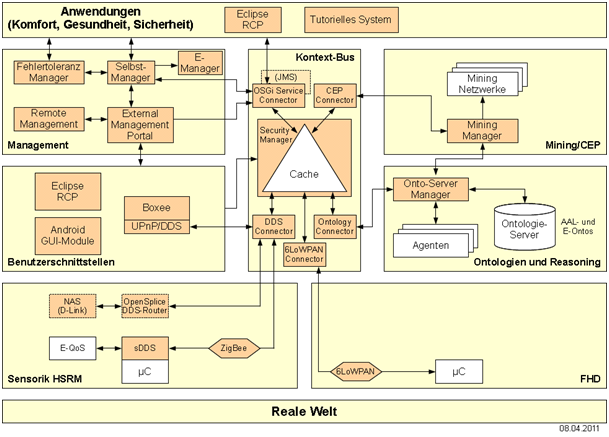
\includegraphics[scale=0.8]{images/wiedas_plattform}
\caption{WieDAS-Plattform}
\label{wiedas_plattform}
\end{figure}

Auf die WieDAS-Plattform (Abbildung \ref{wiedas_plattform}) wird von Benutzern über Anwendungen zugegriffen.
Diese Anwendungen steuern Aktoren oder liefern Mess- und Zustandsinformationen von Sensoren.
Für zusätzliche Hilfestellung beim Bedienen der Anwendungen steht in der Architektur ein
tutorielles System bereit.
Die Plattform kann über Fernwartung oder andere verbundene Management-Modulen verwaltet werden.
Weiterhin stellt die Plattform Verwaltungseinheiten für den Betrieb bereit.
Dazu gehört unter anderem das Sicherheits-Management und das anbieten virtueller fehlertolerante
Dienste, welche den implementierten Diensten überlagert sind.

Der Kern der Plattform ist der Kontext-Bus.
Er besteht aus verschiedenen Adaptermodulen (im weiteren Connectoren), welche für die WieDAS-Komponente
entwickelt werden müssen.
Die Zentraleinheit des Busses (im weiteren Cache) lagert die vorliegenden Daten und bietet sie
den angeschlossenen Modulen (Management- und Connectormodule) über eine Schnittstelle an.
Der Kontext-Bus spielt die zentrale Rolle dabei, Geräte die in der homogenen Einsatzumgebung vorkommen, zu
heterogenisieren.

Zur realen Welt liegt die Schnittstelle der Sensorik.
Hier befinden sich Sensoren, welche autarke Messwerte \cite[Plattform]{wiedas} in den WieDAS-Datenraum
befüllen.
Weitere Komponenten der Sensorik sind Aktoren, welche aus dem System heraus angesprochen werden können
und wiederum Aktionen in WieDAS selbst ausführen können.
Durch die Heterogenisierung im Kontext-Bus, soll z.B. der Sensor eines bestimmten Herstellers in der
Lage sein einen Aktor eines anderen Herstellers zu steuern oder mit Informationen zu befüllen.

Die Plattform enthält weitere Module für z.B. Mining und Reasoning, die für die Entwicklung
der Software keine Relevanz besitzen.

\subsection{AAL-Cache}
\label{gru_aalcache}

AAL-Cache ist die zentrale Softwarekomponente des Kontext-Busses des WieDAS-Projekts \ref{gru_wiedas}.

Der Kern des AAL-Cache ist die Speicherung und Erfassung von Gerätedaten aus dem Umfeld.
Damit die herstellerspezifischen Geräte und Protokolle vom AAL-Cache verarbeitet werden können, schreiben
die Softwareentwickler, die mit dem Cache arbeiten, Adaptermodule (im weiteren Connectoren).
Der Cache läuft stets dauerhaft und kann mittels der geschrieben Connectoren, welche für die
Hersteller spezifische Codestücke enthalten, Daten aus der Umgebung erfassen bzw. in diese verbreiten.
Connectoren sind Module, welche entweder zum Startzeitpunkt oder während der Laufzeit geladen werden
können.
Der AAL-Cache stellt für diese eine Schnittstelle bereit, welche wieder beim Starten der Connectoren
verwendet wird, um sich beim AAL-Cache zu registrieren.
Das Programm bedient sich dabei der Möglichkeit unter Linux dynamische Bibliotheken zu laden.

Für jeden Cache-Eintrag speichert AAL-Cache URIs in Form von Tags und binäre anwendungsspezifische Daten.
Die URIs dienen als Schlüssel und Identifikator für Cache-Einträge.
Aus Performancegründen sind die Einträge Maschinenworte.
Weiterhin speichert der Cache einige Metadaten für jedes Datum.
Darunter z.B. die Identifikation des Schreibers, Zeitstempel für die Erstellung und des letzten
Lesezugriffs des Datums, sowie der Energiebedarf zur Erhebung des Werts \cite{aalcache}.
Zum Zwecke der Lesbarkeit des Datums wird weiterhin ein Datentyp-Hint hinterlegt.

Der Cache selbst kann zur Laufzeit mittels der Management-Schnittstelle konfiguriert werden.
Initial kann der Cache mit XML-Datenstrukturen konfiguriert werden.
Darin enthalten sind z.B. Einstellungen bezüglich der Anzahl und Größte von Speicherpools und Anzahl
der bereitgestellten Cache-Einträge \cite{aalcache}.
Management-Module, welche diese Schnittstelle dann verwenden können, sind in der Lage weitere Speicherpools
anzulegen, falls die vorkonfigurierte Anzahl nicht ausreichend sein sollte.

Im aktuellen Code-Repository befinden sich bereits Connectoren für z.B. OSGi, Ontology-Homeautomation,
DDS und sDDS.

\subsection{Beschreibung der Geräte}

\section{HomeMatic}

HomeMatic ist ein Protokoll der Firma eQ-3 und wird in der Haus- und Gebäudeautomation
verwendet.
HomeMatic-Hausautomation bietet verschiedene Geräte für die Hausinstallation und wirbt damit einfach bedienbar,
zuverlässig, sicher und erweiterbar zu sein \cite{homematic_eq3}.
Das Funk-Kommunikationsprotokoll, welches für die Geräte eingesetzt wird, heißt BidCoS®.
Das Protokoll ist bidirektional und bestätigt empfangene Daten, wodurch die Sicherheit
erhöht wurde.
Es bietet jedoch weitere Sicherheitsmerkmale, z.B. die verschlüsselte Kommunikation.
Es wurde speziell für die drahtlose Ansteuerung der Geräte entwickelt \cite{homematic_eq3_faq},
wird jedoch auch für die Kommunikation über Kabelverbindungen genutzt.

\subsection{Hausautomationsgeräte}

Diese Produktserie befasst sich mit der Hausautomationstechnik und wird in mehrere
Kategorien aufgeteilt.
\begin{enumerate}
\item{Zentralen und Gateways}
\item{Sender und Controller}
\item{Sensoren}
\item{Aktoren}
\end{enumerate}

Um eine komfortable Steuerung und Verwaltung der im Haus befindlichen Geräte durchzuführen,
bietet HomeMatic Stationen an, die als Zentrale dienen.
Die Geräte in der HomeMatic-Umgebung können über Funk oder Kabel mit der Zentrale verbunden
werden.
Um die Zentrale nicht zwangsläufig am PC-Arbeitsplatz aufzustellen, bietet HomeMatic weitere
Adapter und Gateways an, um so z.B. Konfiguration mit USB-Sticks vorzunehmen.
Die Konfiguration selbst geschieht dann über das Aufrufen einer Internetanwendung, die
auf der Zentrale läuft.
Dieses Programm wird WebUI genannt \cite{homematic_webui_manual}.

Durch das Verwenden von HTTP und damit auch TCP, ist man auch in der Lage die Zentrale
über das Internet, z.B. durch die Verwendung von Smartphones zu konfigurieren.
Dazu müssen lediglich die Aufrufe aus dem Internet an die Zentrale weitergeleitet werden
(Router-Portforwarding).

HomeMatic bietet zur Ansteuerung von Aktoren moderne Funk-Fernbedienungen mit verschiedener
Anzahl von Tastern, sowie Möglichkeiten Taster in Gebäude-Elektroinstallationen Unterputz anzubringen.
Um automatisch Werte aus der Hausinstallation zu erfassen, gibt es verschiedene Sensoren für z.B.
Wetter, Rauch, Bewegung und elektrische Impulserkennung.
Als Aktoren dienen Dimmer, Unterputzeinsätze für vorhandene Installationen, einfache Ausgangsmodule und
komplexe Steuerungsmodule für z.B. Heizung oder Türgriffe.

\subsection{XML-RPC}
\label{gru_xmlrpc}

XML-RPC ist der Begriff für einen entfernten Prozeduraufruf unter der Benutzung von XML.
Es baut, wie der Name verrät, auf dem weit verbreiteten und anerkannten Interprozessprotokoll RPC
(Remote Procedure Call).
Wie der Begriff verrät, findet man RPC in verteilten Systemen, wo der Aufrufer eine gewisse
Aufgabe ausgeführt haben möchte und einen Aufruf an ein System absendet.
Der Aufrufer oder Sender wird Client und das System, welches die Aufgabe ausführt Server genannt.


Für den Programmierer ist der Aufruf selbst nicht von einem lokal ausgeführten Aufruf zu unterscheiden.
Der Programmierer sorgt lediglich für den Verbindungsaufbau zum Server.
Die Transportmechanismen sind dabei vom Programmierer versteckt und befinden sich in den jeweiligen
Implementierungen.
Für den Transport zwischen den Teilnehmern werden Nachrichten genutzt, dadurch muss die Implementierung
eine Kodierung (sogenanntes Marshalling) vornehmen.

Für dieses Marshalling bzw. den Transport selbst kann XML verwendet werden.
XML-RPC jedoch ist ein eigenständiges Protokoll, welches ein gewisses Nachrichtenformat erwartet und keine
anwendungsspezifischen Datentypen erlaubt.
Somit müssen Daten mit den vom Protokoll spezifizierten Datentypen strukturiert werden.

Während bei einer Verwendung von XML für RPC der Transportmechanismus keine Rolle spielen würde, findet
der Aufruf eines XML-RPC über HTTP statt.
Dadurch müssen die Clients und Server das HTTP Protokoll implementieren.
Ein Vorteil, welcher auch gleichzeitig ein Nachteil sein kann, ist die Einsehbarkeit der Kommunikation
von beteiligten Systemen.
Um diesem Sicherheitsmangel entgegen zu wirken, wäre eine Kommunikation über HTTPS denkbar.

\chapter{Analyse}
\label{analyse}

Das Hauptziel der zu entwickelnden Software ist die Bereitstellung und Verwendung von HomeMatic-Hausautomationsgeräten
im WieDAS-Datenraum.
Im vorherigen Kapitel wurden die Eigenschaften der verwendeten Komponenten, die in der Entwicklung berücksichtigt werden müssen,
beschrieben.
Wie im Abschnitt \ref{gru_aalcache} bereits aufgeführt, wird der WieDAS-Datenraum (Abschnitt \ref{gru_wiedas_daten})
über eine Instanz einer Cache-Software bereitgestellt.
Die HomeMatic-Geräte (Abschnitt \ref{gru_hm_obj}) sind über eine Zentralkomponente (Abschnitt \ref{gru_hm_ccu}) mit dem Verarbeitungssystem verbunden.
Es wird ein Connector entwickelt, der die HomeMatic-Geräte an den Cache koppelt und bestimmten Anforderungen
gerecht werden muss.
In der Analyse ergeben sich die Problemfelder aus den Anforderungen.
Für diese Problemfelder werden Lösungsansätze und Alternativen vorgeschlagen, sowie ihre Vor- und
Nachteile aufgezeigt.
Danach wird der Entwicklungsprozess des Connectors beschrieben und welche Maßnahmen notwendig sind, um den Connector
im Zielsystem zur Ausführung zu bringen und ihn entsprechend zu konfigurieren.

\section{Anforderungen}
\label{ana_anforderungen}

Für die Analyse wurden die folgenden Kern-Anforderungen für den Connector spezifiziert:
\begin{enumerate}
\item Der Connector muss in der Lage sein, das Anmelden und Abmelden von Geräten zu erkennen, um diese
nicht länger im Verarbeitungssystem zu betrachten
\item Gerätefunktionen müssen wahrgenommen werden, so dass sie in den WieDAS-Datenraum eingepflegt
werden können
\item Bei Änderungen im WieDAS-Datenraum muss der Connector dafür sorgen, dass die entsprechende
Gerätefunktion beim HomeMatic-Gerät durchgeführt wird
\item Es werden Verknüpfungen zwischen verschiedenen WieDAS-Daten erstellt. Der Connector muss
eine Möglichkeit bieten diese anzulegen.
\item Da es stetig mehr HomeMatic-Geräte mit neuen Kanaltypen gibt, soll der Connector in der Lage
sein, zu einem späteren Zeitpunkt neuartige Geräte dynamisch zur Laufzeit des Connectors anzulernen.
\item Durch die Verknüpfung der Geräte bietet sich ebenfalls die Möglichkeit, den Connector in heterogenen
WieDAS-Umgebungen lauffähig zu machen und dort auf Geräteaktionen zu reagieren, die von anderen
Connectoren in den Cache geschrieben werden.
\end{enumerate}

Aus den Kern-Anforderungen und der Ausarbeitung der Grundlagen in Kapitel \ref{grundlagen}
gehen weitere funktionale Anforderungen hervor.
Für das Anlernen von Geräten muss der Anwender auf eine Prozedur zurückgreifen, die in
der Beschreibung der Geräte vorliegt.
Es muss analysiert werden, ob Alternativen zu dieser Prozedur angeboten werden oder
realisierbar sind.
Der Connector wird nach der Anmeldung mittels der angebotenen XML-RPC-Schnittstelle
\ref{gru_hm_ccu} über neue Geräte informiert und ist somit nur reagierend.
Auch das Reagieren auf und das Auslösen von Ereignissen von HomeMatic-Geräten wird
über die angebotene XML-RPC-Schnittstelle realisiert.
Die korrekte Benutzung der Schnittstelle und das Verhalten in verschiedenen Situationen
muss analysiert werden.
Bei der Betrachtung der Gerätebeschreibungen in Abschnitt \ref{gru_hm_obj} und Abschnitt
\ref{gru_wiedas_daten} stellt sich heraus, dass die Geräte durch die Unterschiedlichkeit
der Datenstrukturen aufeinander abgebildet werden müssen.
Dabei muss der Wertebereich der Datentypen betrachtet werden und analysiert werden, ob
eine reine Datenabbildung ausreicht oder ebenfalls funktionale Elemente erforderlich sind,
um das gewünschte Verhalten zu erzielen.
Gerade in Bezug auf die Möglichkeit, dass ein HomeMatic-Gerät mehrere WieDAS-Funktionalitäten
ausüben kann, muss eine modulare Grundlage für die Abbildung gefunden werden.
Da die abgebildeten HomeMatic-Geräte dann auch in WieDAS übertragen werden sollen,
muss analysiert werden, wie sie im AAL-Cache identifiziert werden können.
Diese Information muss dann auch verwendet werden, um von Ereignissen aus dem AAL-Cache
das korrekte HomeMatic-Gerät anzusprechen.
Um dem System unbekannte Gerätetypen zur Laufzeit bekannt zu geben, benötigt es einer Geräteverwaltung.
Die Geräteverwaltung muss in diesem Fall benachrichtigt werden und entsprechend die Gerätedaten laden.
Um Verknüpfungen zwischen verschiedenen HomeMatic-Geräten herzustellen, kann man die
HomeMatic-Zentrale nutzen oder schon im Anmeldungsprozess der Geräte eine Verknüpfung herstellen.
Der Connector soll aber auch in heterogenen Umgebungen mit verschiedenen Connectoren
agieren.
Damit Verknüpfungen in heterogenen Umgebungen erstellt werden können, müssen diese
auf WieDAS-Ebene durchgeführt werden.
Daher muss analysiert werden, ob alle WieDAS-Daten verarbeitet werden können.
Es muss analysiert werden, wie das System diese Verknüpfungen herstellen kann und wie die
Möglichkeit dem Anwender angeboten wird.
Dadurch, dass der Connector in eingebetteten Systemen verwendet wird, müssen nicht-funktionale Anforderungen erfüllt werden:
\begin{enumerate}
\item geringe Speichernutzung
\item kleinere, leicht optimierbare Subroutinen
\item Verzicht auf komplexe Datenstrukturen, die den Connector unnötig vergrößern
\item Energieeffizienz (in Bezug auf Threading, Polling, Sleep-State, usw.)
\end{enumerate}

\section{Anwendungsfälle}
\label{ana_uc}

Für die Anwendungsfälle wird davon ausgegangen, dass der Connector im Zielsystem ausgeführt wird
und das System zur Verarbeitung bereit ist.
Der Anwender interagiert also mit dem voll funktionsfähigen System.
Das bedeutet unter anderem, dass
\begin{itemize}
\item Die Netzwerkeinstellungen korrekt sind
\item Der Connector in der Konfigurationsdatei korrekt eingetragen wurde (Abschnitt \ref{gru_aalcache})
\item Der Connector die in der Umgebung vorhandenen Geräte verarbeiten kann
\item Die Verknüpfungen mit der bereitgestellten Möglichkeit hergestellt hat
\item Die notwendigen Informationen zur An- und Abmeldung der Geräte im Besitz des Anwenders sind
\end{itemize}

\myfigurescaled[0.5]{h}{uc}{Anwendungsfälle}

\subsection{Geräte bei HomeMatic-Zentrale an- und abmelden}
\label{uc1}
Der Anwender muss in der Lage sein die Geräte an- und abzumelden.
Dazu wird die Anmeldungsprozedur der Gerätebeschreibung entnommen und an der HomeMatic-Zentrale
durchgeführt.
Der Connector muss diese Anmeldung erkennen und eine interne Abbildung laden.
Bei einer Abmeldung muss das Gerät wieder aus dem Speicher entladen bzw. gelöscht werden und
die Verarbeitung von Verknüpfungen und Behandeln von Ereignissen einstellen.
Eine Statusmeldung informiert den Anwender darüber, ob eine An- oder Abmeldung registriert wurde.

\subsection{Funktionen an HomeMatic-Geräten auslösen und im Connector erkennen}
\label{uc2}
Der Anwender kann Funktionen an einem HomeMatic-Gerät durchführen und diese dann
im AAL-Cache als WieDAS-Datenobjekt wiederfinden, falls das Gerät vom Connector
unterstützt wird.
Dazu kann der Connector eine Statusmeldung geben, sobald ein Ereignis von der HomeMatic-Zentrale
geliefert wurde.

\subsection{HomeMatic-Geräte mit anderen Geräten im WieDAS-Datenraum verknüpfen}
\label{uc3}
Weiterhin will der Anwender Verknüpfungen zwischen verschiedenen Geräten im WieDAS-Datenraum herstellen.
Dabei sollen sowohl HomeMatic-Geräte untereinander, als auch HomeMatic-Geräte mit anderen Geräten
verknüpft werden.
Ein HomeMatic-Gerät kann als Sensor dienen und ein anderes Gerät im WieDAS-Datenraum als Aktor oder umgekehrt.
Die Art und Weise, wie diese Verknüpfung erzeugt wird, ist offen.
Der Aufwand für die Erstellung der Verknüpfung soll im überschaubaren Rahmen liegen und
dokumentiert werden.
Der Benutzer eines anderen Connectors ist in der Lage, mittels der hier entwickelten Geräteabbildung
Verknüpfungen mit den HomeMatic-Geräten herzustellen.

\section{Verwaltung der Gerätemengen}
\label{ana_gemenge}
WieDAS-Datenobjekte sind im Grunde nur Datenvariablen mit Schreib- und Lesefunktionen (Abschnitt \ref{gru_wiedas_daten}).
Sie besitzen wenig Attribute und lassen wenig Spielraum bei der Interpretation der Daten.
Die Recherche im Dokument für Datenpunkte der HomeMatic-Geräte \cite{hmscript4} ergab keinen
Bedarf für eine Abbildung von einer einzelnen Funktion zu mehreren HomeMatic-Geräten.
Dennoch ist es möglich, dass z.B. eine Verknüpfung erstellt wird, wo 2 Taster gleichzeitig
gedrückt werden müssen, um eine Steckdose zu schalten (z.B. aus Sicherheitsgründen).
Sollte diese Art der Verknüpfung erwünscht sein, muss beachtet werden, dass die Ereignisse
dem Connector zeitlich versetzt mitgeteilt werden können.
Dadurch muss der Connector, falls ihm durch das Callback nur das Drücken eines Tasters
mitgeteilt wird, prüfen, ob der andere ebenfalls gedrückt wurde.

In Abschnitt \ref{gru_hm_obj} wird erwähnt, dass HomeMatic-Geräte die Möglichkeit besitzen,
mehrere Funktionen mit einem einzigen Gerät auszuführen (Beispiel Thermostat).
Deshalb muss untersucht werden, welche HomeMatic-Geräte in der Lage sind, welche Funktionen
auszuüben.
Für den Entwurf bzw. die Implementierung sollten alle zur Verfügung stehenden Geräte
berücksichtigt werden, um auch evtl. mehrere Gemeinsamkeiten zu finden und die Geräte
besser modellieren zu können.
Die Unterstützung von mehreren WieDAS-Funktionalitäten in einem einzigen Gerät hat zudem
zur Folge, dass beim Entwickeln der Geräte-Abbildung berücksichtigt werden muss, dass mehrere
URIs auf ein HomeMatic-Gerät zugreifen werden.
Die genaue Abbildung der URIs wird in den Geräteabbildungen näher analysiert.

Um dem System mitzuteilen, welche Geräte vorhanden sind, müssen diese am System angemeldet werden.
Bei Funktionen aus dem WieDAS-Datenraum besteht keine Notwendigkeit, die Geräte anzumelden.
Sie werden durch den Connector, der die Daten bereitstellt angemeldet.
Durch die Verwendung von AAL-Cache (Abschnitt \ref{gru_aalcache}) kann das Datenobjekt
direkt vor dem ersten Einfügen in den Cache \emph{registriert} werden.
Dazu muss nur ein Tag vom Cache angefordert werden, was immer durchgeführt wird, sobald
ein Datum in den Cache hinzugefügt wird.
Der Tag dient zur resourcenschonenden Identifizierung des URI (Abschnitt \ref{gru_aalcache})
und kann jederzeit wieder durch den AAL-Cache zurück in den URI umgewandelt werden.
Eine Abmeldung bzw. Löschung eines Tags aus AAL-Cache muss nicht durchgeführt werden.
AAL-Cache verdrängt die Tags nach dem \emph{Least-Recently-Used}-Verfahren \ref{gru_aalcache}.
Um auf Änderungen im WieDAS-Datenraum zu reagieren, müssen die abgebildeten HomeMatic-Geräte
mitteilen, für welche URIs sie Benachrichtigungen erhalten wollen.
Mit den bekannten URIs kann die Registrierung eines Callbacks durchgeführt werden.
Dieses Callback liefert dann bei Aufruf die veränderten Tags (und dadurch auch die URIs),
und der Connector kann die entsprechenden Geräte benachrichtigen.
Eine Alternative, um die Modellierung zu entschlacken, wäre das Ablegen aller URIs, die
für irgendein HomeMatic-Gerät interessant sein könnte, in einer Datei.
Diese könnte dann vom Connector gelesen werden und jegliches Ereignis zu einem dieser
URIs würde dazu führen, dass jedes Gerät selbst entscheidet, ob es diesen URI
verarbeiten kann.

Bei HomeMatic werden Geräte zunächst der Zentrale bekannt gegeben (Abschnitt \ref{gru_hm_ccu}).
Die Art- und Weise, wie der Anmeldungsprozess vollzogen wird, hängt dabei stark vom Gerät ab.
Beim Durchlesen der Beschreibungen für verschiedene Geräte (insb. Dimmer und Wandtaster)
konnte man feststellen, dass es verschiedene Anmeldungsprozesse gibt.
Zum Beispiel können im Anlernmodus Geräte direkt miteinander verknüpft werden \cite[Seite 6]{hmdimmer}.
Bei ersten Versuchen hat sich herausgestellt, dass die direkte Verbindung dazu führt, dass
die Ereignisse nicht weiter über die externe Schnittstelle weitergeleitet werden.
Geräte können auch über den Schnittstellenprozess der HomeMatic-CCU mit dem Aufruf von \emph{addDevice}
\cite[Seite 16]{homematic_webui_manual} angemeldet werden.
Dazu wird eine Seriennummer benötigt.
Dies wird aber nur für einige Geräte unterstützt.
Bei erfolgreicher An- und Abmeldung wird dem Logikprozess (Abschnitt \ref{gru_hm_ccu}) die Liste
der involvierten Gerätebeschreibungen mitgeteilt.
Um einen Abgleich der Gerätebeschreibungen zuzulassen (Abschnitt \ref{gru_hm_ccu}),
kann ein kleiner Teil der Beschreibungen für die bekannten Geräte gespeichert werden.
Bei einem Ereignis wird die Adresse des logischen Geräts mitgeteilt.
Wird bei einem Zugriff von der Zentrale auf ein HomeMatic-Gerät zugegriffen, so muss eine interne
Assoziation von Adresse zur richtigen Abbildung gespeichert werden.
Wird durch ein Ereignis aus dem WieDAS-Datenraum auf ein HomeMatic-Gerät
zugegriffen, so muss entweder die Zentrale nach der Gerätebeschreibung für die Adresse abgefragt werden
oder durch den Erhalt der Adresse aus dem URI auf die interne Assoziation zugriffen werden.

%Die Abbildung mehrerer WieDAS-Funktionen auf ein Gerät ist Bestandteil der folgenden Analyse.
Bei der Entwicklung des Connectors müsste eine Proxy-Anwendung entwickelt werden, die die
Befehle für eine Anmeldung ausführt und auf dem System läuft, auf dem sich der Connector befindet.
Für andere Geräte müsste auf die Anmeldung an der Zentrale zurückgegriffen werden.
Aufgrund des hohen Mehraufwands wird bei der Entwicklung die Anmeldung der Geräte durch einen
Benutzer nicht einbezogen und ist alleinige Aufgabe des Anwenders.
Um Funktionen im WieDAS-Datenraum entsprechend der Geräte anzubieten und umgekehrt wird ein URI benutzt.
Damit der Connector die richtige Geräteabbildung findet, wird beim Entwurf auf ein Mapping
von Geräte- und Kanaladresse zur Abbildung gespeichert.
Eine Abbildung von einer WieDAS-Funktionalitäten auf mehrere HomeMatic-Geräte wird durch die
Designentscheidungen möglich gemacht, jedoch nicht exemplarisch entworfen, da dafür keine
Geräte im Rahmen der Entwicklungsphase zur Verfügung stehen.
Der Logikprozess speichert die notwendigen Gerätebeschreibungen für die HomeMatic-Zentrale, um
ihr einen Abgleich zu erlauben, da die Liste nur wenig Speicher verbrauchen wird.
Die Verknüpfungen zwischen verschiedenen Geräten im WieDAS-Datenraum wird über das Erstellen
dynamischer Bibliotheken realisiert.
Das gleiche Prinzip wird angewandt, um Geräte zu laden.
Die Geräte werden in dynamischen Bibliotheken abgebildet und decken jeweils das Laden der Geräte
einer Typenreihe ab.
Diese werden bei Programmstart geladen und können bei Bedarf aus einem Verzeichnis nachgeladen werden.
Um die Bibliotheken nachzuladen, muss ein Signal an den Connector geschickt werden.

\section{Abbildung der Geräte}
\label{ana_abbildung}
Die Kernanalyse beschäftigt sich mit der Abbildung von HomeMatic-Geräten und WieDAS-Funktionen.
HomeMatic-Geräte sind im Grunde ein Container für mehrere Kanäle (Abschnitt \ref{gru_hm_obj}).
Die Datenpunkte und Kanäle eines einzelnen Geräts sind leider nicht in den Beschreibungen
der Geräte spezifiziert, sondern müssen dem Dokument für Datenpunkte \cite{hmscript4} entnommen werden.
Im Grunde sind die meisten Datenpunkte selbsterklärend (\emph{PRESS\_SHORT}, \emph{PRESS\_LONG}, usw.)
jedoch gibt es einige Datenpunkte, wo eine Beschreibung sinnvoll wäre (\emph{INSTALL\_TEST}, \emph{INHIBIT}, usw.).
Man könnte sich vorstellen, dass ein Kanaltyp (z.B. \emph{Key}) oder ein Datenpunkt immer genau für eine
WieDAS-Funktion verwendet werden kann.
Jedoch würde diese 1:1 Verknüpfung keinen Sinn ergeben.

\myfigurescaled[0.45]{h}{taster}{Mögliche Abbildungen eines HomeMatic-Tasters in WieDAS}

Abbildung \ref{abb_taster} zeigt 2 verschiedene Möglichkeiten einen Taster in WieDAS abzubilden.
Ein Taster besitzt 2 Kanäle vom Kanaltyp \emph{Key} (hier: \emph{K1} und \emph{K2}).
Der Kanaltyp besitzt jeweils die Datenpunkte \emph{PRESS\_SHORT}, \emph{PRESS\_LONG} und
\emph{PRESS\_CONT} \cite{hmscript4} (jeweils vom Datentyp: \emph{BOOL}).
Nun gibt es die Möglichkeit, den Taster entweder so abzubilden, dass ein Kanal der WieDAS-Funktionalität
zugeordnet wird.
Dazu müsste ein kurzer Tastendruck auf einer Seite des Tasters dafür sorgen, dass in der WieDAS-Funktionalität
die Werte \emph{on} oder \emph{off} gesetzt werden und bei einem langen Tastendruck auf der gleichen Seite
des Tasters der entsprechend andere Wert.
Eine andere Möglichkeit ist es, den Taster so abzubilden, dass ein kurzer Tastendruck auf einer Seite
die Funktionalität \emph{on} und ein kurzer Tastendruck auf der anderen Seite das Attribut in der
WieDAS-Funktionalität auf \emph{off} setzt.
Beim Entwurf der Geräte können beide Möglichkeiten berücksichtigt werden.
Dadurch ist es möglich, dass ein Taster (mit 2 Druckzuständen pro Seite) 2 WieDAS-Funktionen anbieten kann.
Das Beispiel verdeutlicht auch, dass es keine allgemeine Abbildungsvorschrift gibt.
Die Geräte müssen einzeln entworfen und implementiert werden.
Es kann jedoch beim Entwurf schon für beide Szenarien eine entsprechende Abbildung unter einem anderen
Namen erstellt werden (z.B. Taster und Taster-2).

%TODO KROEGER (allgemeiner, wenn vorher cache-einträge als structs formal dann hier z.b. id, typ, etc.)
Geräte müssen in der Lage sein die angebotenen Funktionalitäten in URIs zu beschreiben.
Eine Möglichkeit, die URIs zu formen, ergibt sich aus der WieDAS-IDL \cite{wiedas_idl}
und den verschiedenen Kanälen und deren Typen.
Die Identifikation von HomeMatic-Geräten geschieht über Adressen (Abschnitt \ref{gru_hm_obj}).
Um der URI eine Information zukommen zu lassen, dass es sich um ein Gerät der HomeMatic-Produktserie,
kann dem URI eine Zeichenkette hinzugefügt werden.
Dies ist nicht zwingend erforderlich, hilft aber dabei, die einzelnen Geräte im WieDAS-Datenraum
zu unterscheiden.
Eine weitere Möglichkeit wäre es, dem URI den Aufenthaltsort des Geräts mitzuteilen, jedoch kann
dadurch bei Auftreten eines Ereignisses nicht direkt herausgefunden werden, welches Gerät
an einem Ort gemeint ist (Beispiel: 2 Taster in der nähe eines Türrahmen), sie müssten zusätzlich
mit einem Index versehen werden.
Weiterhin könnten Aufgaben als Identifikator benutzt werden.
Für die beiden letzten Abbildungsmöglichkeiten bedarf es der Speicherung einer Abbildung
von Aufenthaltsort/Funktion zur eigentlichen Adresse.

\begin{table}[h]
\begin{tabular}{|l|l|l|l|l|}
\hline
Gerät & Kanal\# & Aufgabe & Ort & URI \\
\hline
ABC123 & 1 & Licht & Schlafzimmer & /OnOffFunctionality/HMABC123-1 \\
\hline
ABC123 & 1 & Licht & Schlafzimmer & /OnOffFunctionality/Schlafzimmer1 \\
\hline
ABC123 & 1 & Jalousie & Schlafzimmer & /OnOffFunctionality/Jalousie1 \\
\hline
\end{tabular}
\caption{Möglichkeiten der URI-Abbildung}
\label{tab_abb_uri}
\end{table}

Tabelle \ref{tab_abb_uri} zeigt Möglichkeiten für die Abbildung von URIs.

Da die Hashing-Funktion für die Erzeugung von Tags aus URIs in AAL-Cache eine breite
Verteilungsfunktion besitzt (Abschnitt \ref{gru_aalcache}), hat die Wahl des URI
keine Konsequenzen in Bezug auf Speichernutzung, weil z.B. zu viele Tags entstehen könnten.

Es gibt 2 verschiedene Verwendungen der Abbildungen.
Für die Identifikation der 2 benötigten Verwendungen dient der URI.
Eine Abbildung wird benötigt, sobald ein HomeMatic-Ereignis, durch Aufruf der
\emph{event}-Funktion (Abschnitt \ref{gru_hm_ccu}) dem Connector unter Verwendung
der Logikschnittstelle mitgeteilt wird.
Wie bereits im Abschnitt \ref{ana_gemenge} ermittelt, wird ein Mapping der Geräte gespeichert.
Daher ist es wichtig zu wissen, welche Informationen für das korrekte Abbilden für das
Gerät benötigt werden.
Eine unnötige Ansammlung von zu vielen Daten für ein Gerät hat einen großen Anstieg
des benötigten Speicherbedarfs zur Folge.
Eine Alternative wäre, die nötigen Informationen von der Zentrale abzurufen, sobald
sie für das Ausführen von verschiedenen Funktionen benötigt werden.
Wird ein Ereignis ausgeführt, gibt es die Möglichkeit, die Daten für das Gerät zusammen
mit einer ``Verhaltensregel'' für entsprechende Daten aus dem Mapping zu erhalten oder
man bestückt den Geräteentwurf mit Funktionen, welche dann auf den eigenen
Daten agiert.

Eine 2. Verwendung für die Abbildung erfolgt, wenn der AAL-Cache das Datum der Funktionalität
erneuert und dem Connector über das registrierte Callback dies mitteilt (Abschnitt \ref{gru_aalcache}).
Die WieDAS-Funktionen besitzen zusätzlich noch eine ID für die eindeutige Identifizierung
im WieDAS-Datenraum (Abschnitt \ref{gru_wiedas_daten}), welche aber nicht benötigt wird.
Um trotzdem eine gewisse Eindeutigkeit zu erreichen, wie es die WieDAS-IDL
für dieses Attribut vorsieht, können Teile der Adresse, z.B. Hash oder
Ausschnitte davon benutzt werden.
Um die IDL bzw. die spezifizierten Datentypen für den Connector zugänglich zu machen, muss die
WieDAS-IDL-Datei für die verwendete Programmiersprache angepasst werden.
Dafür existieren eine Reihe von IDL Präprozessoren.
Es kann jedoch auch ein eigener Präprozessor geschrieben werden oder die Umwandlung manuell
durchgeführt werden, um Abhängigkeiten zu anderen Projekten zu vermeiden.
Durch Verwendung der IDL in anderen Connectoren ist der Connector in der Lage, bei ihnen
Gerätefunktionen auszulösen oder von ihnen zu empfangen.
Damit das Gerät auf eine Änderung im WieDAS-Datenraum reagieren kann, müssen die URIs,
die das Gerät identifizieren, registriert werden.
Daher muss für die Abbildung der URI oder die URIs gespeichert werden und dem Connector
bei der Registrierung der Callback-Funktionen zur Verfügung gestellt werden.
Damit das Gerät dann weiß, um welches WieDAS-Datenobjekt es sich handelt, muss der URI
der Verarbeitung des Ereignisses übergeben werden.

Für das Design habe ich mich entschieden, dass die Geräte durch ihre starke Abweichung von den
Funktionen der WieDAS-Geräte funktional auf die eintretenden Ereignisse reagieren und die
Verarbeitung nicht mittels Daten und Verhaltensregel an eine Verarbeitungskomponente delegiert.
Es wird jedoch ein Generator entwickelt, um die Deklarationen und Verarbeitungsschritte, die immer
benötigt werden, nicht jedes mal neu schreiben zu müssen.
Dieser Generator hilft dann die in Abschnitt \ref{ana_gemenge} angesprochenen dynamischen
Bibliotheken zu erstellen.
Die Geräte selbst speichern die Informationen, die sie zum Verarbeiten der Ereignisse
benötigen, da für das Abrufen der Informationen von der Zentrale zu viel Zeit verloren geht.
Die URIs werden aufgrund der Einfachheit aus der WieDAS-Funktionalität, einer Zeichenkette,
der Adresse und einer ID zusammengesetzt.
Die Zeichenkette dient als Indikator, dass es sich um HomeMatic-Geräte handelt.
Die ID ist für die interne Verwendung der Geräte (z.B. Bündelung von Kanälen).

\section{Verwendung der Schnittstellen}
\label{ana_schnitt}
Der Connector verwendet im wesentlichen 2 Schnittstellen.
Die Schnittstelle zur Anbindung an die HomeMatic-Zentrale (Abschnitt \ref{gru_hm_ccu} und
für die Interaktion mit AAL-Cache (Abschnitt \ref{gru_aalcache}).

Die HomeMatic-Zentrale kommuniziert mit dem Connector über das XML-RPC-Protokoll (Abschnitt \ref{gru_xmlrpc}).
Um das XML-RPC-Protokoll zu benutzen, muss ein XML-RPC-Client eingesetzt werden, der die
Nachrichten erstellt und abschickt.
Der XML-RPC-Client kann dabei synchron oder asynchron arbeiten.
Der Client muss, durch die Forderung des Protokolls, als Transportprotokoll HTTP nutzen.
Eine Alternative, um dies zu unterbinden, wäre die Kommunikation über HTTP über SSL.
Wie in Abschnitt \ref{gru_hm_ccu} bereits erklärt wurde, steht als einzige Sicherheitsmaßnahme für die
Zugriffsrestriktion auf die Schnittstelle die Möglichkeit die IP-Adressen anzugeben, welche Zugriff bekommen.
Dadurch ist die Kommunikation zwischen der HomeMatic-CCU und dem Connector vollständig einzusehen
und manipulierbar.
%TODO DANIEL (strich zwischen Der und Client)
Der Client ist dafür zuständig, die Funktionen, die im XML-RPC-Dokument von HomeMatic \cite{homematic_xmlrpc}
hinterlegt sind, für den Connector zugänglich zu machen.
Die verschickten Nachrichten bestehen vollständig aus Text.
Da die Nachrichten einem bestimmtem Format entsprechen (Abschnitt \ref{aufbau_xmlrpc}) kann
ein Template benutzt werden, um nur die entsprechenden Werte für den Aufruf einzufügen.
Dabei müssen Konvertierungen von Datentypen und Datenstrukturen vorgenommen werden.
Das bedeutet, dass ein Modul entworfen werden muss, welches die Datentypen aus der XML-RPC-Schnittstellenbeschreibung
von HomeMatic in verwertbare Datentypen für den Connector umwandelt.
Gleichzeitig muss das Modul die verwendeten Typen in Text umwandelt, um sie mit XML-RPC über das Netzwerk zu schicken.

Ein wichtiger Bestandteil beim Arbeiten mit dem Client ist das Behandeln von Fehlern beim Empfangen oder
Senden von Nachrichten.
Tritt ein Fehler beim Senden von Nachrichten auf, so sollte der Connector in der Lage sein dies abzufangen
und zu ignorieren.
Ein Abschalten des Connectors bei einer geringen Netzwerkstörung oder bei Fehlfunktion der HomeMatic-Zentrale
wäre nicht angemessen.

Die HomeMatic-CCU stellt 3 XML-RPC-Schnittstellenprozesse zur Verfügung (Abschnitt \ref{gru_hm_ccu}), jedoch werden
bei der Entwicklung des Connectors nur drahtlos angebundene Geräte berücksichtigt, wodurch der Connector
nur mit einem Schnittstellenprozess kommunizieren muss.
Ein Client alleine reicht jedoch nicht, um den Anforderungen gerecht zu werden.
Da auf Ereignisse aus der Zentrale reagiert wird, muss der Connector eine Logikschnittstelle (Abschnitt \ref{gru_hm_ccu})
bereitstellen.
Dazu muss ein XML-RPC-Server im Connector ausgeführt werden.
Der Server sorgt dafür, die nötigen Methoden, die im XML-RPC-Dokument von HomeMatic \cite{homematic_xmlrpc} angegeben sind,
anzubieten.
Die Methoden können dann entweder direkt auf die Ereignisse bzw. Aufrufe reagieren oder aber das Warteschlangenprinzip
nutzen, welches auch vom AAL-Cache benutzt wird.
Dazu könnten einfache Datenstrukturen verwendet werden, die den Namen des Aufrufs und die übergebenen Daten kurzzeitig
speichern.
Der Connector kann dann, sobald er in einen Idle-Zustand verfällt, die relevanten Datenstrukturen betrachten und
die entsprechende Arbeit verrichten.
Falls der Server einen Fehler bei der Verarbeitung des Requests feststellt, so muss er dies dem Aufrufer mitteilen
(Abschnitt \ref{aufbau_xmlrpc}).
Der Schnittstellenprozess hat für Fehler in der XML-RPC-Nachricht entsprechende Fehlercodes definiert (Abschnitt \cite{homematic_xmlrpc}).
Da der Server ständig auf Ereignisse warten muss, ist es notwendig, ein Polling, also eine Abfrage für eingehende
Nachrichten, durchzuführen oder auf eingehende Nachrichten in einem Thread oder Prozess zu warten.

Der AAL-Cache verwendet eine rudimentäre C-Schnittstelle, um auf den Kern zugreifen zu können (Abschnitt \ref{gru_aalcache}).
Beim Eintragen von WieDAS-Daten in den Cache verwendet das Gerätemodell (Abschnitt \ref{ana_abbildung}) die Funktionalität
zum Einfügen von Daten.
Ein größerer Aspekt ist die Verwendung der Callback-Funktionalität von AAL-Cache.
AAL-Cache stellt für die Registrierung eines Callbacks eine Funktion bereit.
Ihr wird mitgeteilt, wie viele Tags und welche Tags beobachtet werden sollen.
Eine Möglichkeit wäre es, den Gerätemodellen die Registrierung ihrer URIs zu überlassen.
Dies würde allerdings zu einem starken Anstieg des Speichverbrauchs führen, da für jede Registrierung eine
Datenstruktur aufgebaut wird (\emph{SubscriptionSet-Handle}) und im AAL-Cache gespeichert wird.
Eine Alternative ist das Registrieren aller gewünschten Tags in einem einzigen \emph{SubscriptionSet}.
Dann müsste der Connector dafür sorgen die URIs, welche im Callback mitgeteilt werden, den Geräten zuzuordnen
und die Geräte darauf reagieren zu lassen (Abschnitt \ref{ana_abbildung}).
Callbacks werden in Threads ausgeführt und man darf keine Annahmen über den Thread treffen, in dem das
Callback aufgerufen wird \cite{aalcache}.
Dadurch das der XML-RPC-Server für das Abarbeiten der Methodenaufrufe (s.o.) ebenfalls Threads oder ähnliches
benutzen muss, müssen Vorkehrungen getroffen werden um geteilte Datenstrukturen zu schützen.
Wie schon bereits im vorherigen Absatz erläutert, benutzt AAL-Cache ein Warteschlangenprinzip zum Einreihen
der Callback-Funktionen.
Um die Abarbeitung im gleichen Prozesskontext bzw. Thread durchzuführen, kann hier wiederum das gleiche
Prinzip angewandt werden.
Das Callback kann die nötigen Abarbeitungen einreihen und im gleichen Kontext ausführen, wie die restlichen
Aufgaben.

Für den Entwurf der Schnittstellenabbildung habe ich entschieden die XML-RPC-Bibliothek \emph{xmlrpc-c} \cite{xmlrpc-c} zu verwenden.
Diese bietet eine Client- und Serverimplementierung, sowie nötige Hilfsmittel zur Generierung von Nachrichten und
 ist durch die Verwendung von C geeignet den Connector ohne Hinzufügen von weiteren Abhängigkeiten zu unterstützen.
Ein striktes Binden an ein Kommunikationsmodell des Clients (synchron oder asynchron) ist anhand der Analyse nicht nötig.
Die Bibliothek bietet sowohl asynchrone als auch synchrone Schnittstellenaspekte an.
Die Serverimplementierung wird allerdings nur synchron angeboten.
Da die Verwendung der asynchronen Client-Schnittstelle jedoch die Komplexität, durch Verwendung von Betriebssystem-abhängigen
Netzwerkschnittstellen, in den Connector einbringen würde, wird die synchrone Schnittstelle verwendet.
Da der Sicherheitsaspekt bei der Kommunikation nicht gefordert wurde, ist es hier nicht nötig, Rücksicht auf die
beschrieben Problematik bezüglich der Sicherheitsprobleme bei ungesicherter Übertragung zwischen den Komponenten zu nehmen.
Diese wären Bestandteil der Analyse einer Weiterentwicklung des Connectors.
Es existieren für die Bibliothek Möglichkeiten, XML-RPC über HTTPs zu übertragen \cite{xmlrpc_ssl}.
Da die Bibliothek sich intern um die Struktur der Nachrichten für Requests und Antworten kümmert, müssen die
analysieren Fehlerbehandlungen auf Protokollebene nicht weiter beachtet werden, da sie abstrahiert werden.
Trotzdem muss darauf geachtet werden, dass Fehler beim Absetzen von Nachrichten zwar erkannt werden, aber nicht
zur Beendigung des Connectors führen, da kurzzeitige Störungen bei der Kommunikation vernachlässigt werden.
Da die HomeMatic-Zentrale keine Aussagen darüber trifft, ob sie eine Fehlerbehandlung durchführt, sobald
der Logikprozess eine Fehlermeldung zurückliefert, gibt es keine Rückmeldung (\emph{faultCode}-Element)
von Fehlern.
Für die Abarbeitung der Callbacks und der Ereignisse der HomeMatic-CCU kann das angesprochene Warteschlangenprinzip
nicht verwendet werden.
Da der XML-RPC-Server der Bibliothek nicht unterbrochen werden kann, müsste die Abarbeitung des AAL-Cache
Callbacks warten, bis der nächste RPC bearbeitet wird.
Deshalb wird Locking verwendet, um die geteilten Resourcen vor gleichzeitigem Zugriff zu schützen.

\section{Entwicklungsprozess}
\label{ana_entwicklung}

%TODO KROEGER (wohl epic fail)
Der Connector ist eng an den AAL-Cache gekoppelt \cite{aalcache} und durch die Verwendung der XML-RPC-Schnittstelle
von den HomeMatic-Geräten entkoppelt.
Für den Entwurf des Connectors wurden mehrere bereits vorhandene Connectoren im AAL-Cache-Code-Repository \cite{aalcache_code}
betrachtet.
Das Repository enthält die Schnittstellen, die Implementierung, eine Dokumentation, sowie verschiedene Connector-Implementierungen
mit Bauanleitungen.
Die Connector-Implementierung wird in der Umgebung des Code-Repository erfolgen, um ein einfaches Hinzufügen der Implementierung
für zukünftige Weiterentwicklung zu ermöglichen.

Die Bauanleitungen benutzen im wesentlichen ANT-Dateien \cite{ant} und Makefiles \cite{make}.
Das Ergebnis der Verarbeitung der Bauanleitung ist mindestens eine dynamisch ladbare Bibliothek.
Durch das Einbinden der dynamischen Bibliothek in den Connector zur Laufzeit ist der Connector eng gekoppelt.
Die dynamische Bibliothek wird dann in einer Textdatei (\emph{connectors.conf}) eingetragen, so dass der Connector diese
beim Starten laden kann.
Für den Entwicklungsprozess stellt der AAL-Cache eine Debugging-Schnittstelle zur Verfügung, welche durch die Verwendung eines
Makros auch wieder deaktiviert werden kann.

Das Verwenden von dynamischen Bibliotheken hat zur Folge, dass ein UNIX-artiges Betriebssystem (Mac, Linux, BSD, usw.) notwendig
ist, um AAL-Cache zu starten und den Connector zu laden.
Da vorhandene Connectoren und der Cache auf eingebetteten Geräten eingesetzt werden, muss der Connector die nicht-funktionalen
Anforderungen, die in Abschnitt \ref{ana_anforderungen} ermittelt wurden, berücksichtigen.

Um die Speichernutzung gering zu halten, sollten redundante Informationen so weit es geht
verworfen oder reduziert werden, ohne dass die Reaktionszeit des Systems stark beeinträchtigt wird.
Es ist zum Beispiel nicht gewollt, auf einen Schaltbefehl 2 Sekunden lang warten zu müssen,
bis die Lampe erleuchtet, weil das System viele Daten ermitteln muss, um den Schaltbefehl zu realisieren.

Kleinere Subroutinen sind für Compiler aus der Embedded-Umgebung, welche evtl. nicht die
Optimierungsfähigkeiten größerer Compiler besitzen, zu optimieren.
Optimierter Code lässt das System schneller, effizienter und speicherschonender werden.

Da der AAL-Cache dauerhaft auf dem System ausgeführt wird, ist es wichtig, wenig Gebrauch
von globalen Informationen zu machen und stattdessen so viel wie möglich Datenstrukturen
lokal zu halten.
Je nach Servermodell müssen evtl. Sleep-States oder Timeouts benutzt werden, um andere
Prozesse bzw. Threads arbeiten zu lassen, während man selbst auf Ereignisse wartet.

Da der Connector verschiedene Informationen für die Verbindung zur HomeMatic-CCU benötigt,
muss dem Connector die Netzwerkkonfiguration des Systems mitgeteilt werden.
Falls eine Netzwerkverbindung getrennt wird oder die CCU nicht zu erreichen ist, muss der Connector
entsprechend darauf reagieren ohne sich abzustellen.
So muss der Anwender bei kleineren Netzwerkstörungen den Connector nicht neu laden.
Als Alternative kann der Connector beim Initialisieren selbst Netzwerkeinstellungen,
blockierte Ports, usw. mittels der Betriebssystem-API ermitteln.
Um die Logik-Schnittstelle aufzubauen, benötigt die Software einen freien Port und
eine zugewiesene IP-Adresse, an dem der Server bereitgestellt wird.
Aus Sicherheitsgründen können hier Einschränkungen vorgenommen werden bezüglich
der Reichweite der IP-Adresse und der Portnummer.
Da die Software und die Vorgehensweise des \emph{NetFinder} Programms (Abschnitt \ref{gru_hm_ccu})
nicht eingesehen oder erahnt werden kann, muss dem Connector die IP-Adresse und
dem Port der XML-RPC-Schnittstelle der HomeMatic-CCU mitgeteilt werden.
Dies kann durch die Konfigurationsdatei \emph{connectors.conf}-Datei geschehen.
Falls eine enge Kapselung der CCU an das System besteht (z.B. durch ein privates
kleines Netzwerk) muss eine Weiterleitung eingerichtet werden.


%TODO
%- setzt architektur vorraus
%- gedanken vermischt
%- datenstrukturen und abläufe mehr trennen
%- abläufe aus anwendungsfällen ableiten lassen
%- designentscheidungen schwer nachzuvollziehen und nicht sichtbar
%- kaum abbildungen

\chapter{Design}
\label{design}

Dieses Kapitel zeigt den Entwurf des HomeMatic-Connectors für den WieDAS-Datenraum.
Der Entwurf erfüllt die grundlegenden Anforderungen, die im letzten Kapitel
herausgearbeitet wurden und wurde in den Entscheidungen begründet.
Als erstes wird der Entstehungsprozess des Connectors erläutert.
Dann folgt eine Beschreibung der Gesamtarchitektur, in welcher sich der Connector befindet
und eine Kurzbeschreibung der Komponenten mit denen er über verschiedene Kommunikationswege
interagiert.
Komplexere HomeMatic-Gerätedaten, welche vom XML-RPC-Protokoll übertragen und
entsprechend verarbeitet werden müssen, besitzen eine Abbildung in Klassen zur einfacheren
Nutzung, welche anhand von Beispielen beschrieben wird.
Danach wird die Geräteabbildung zwischen HomeMatic und WieDAS, die aus (Abschnitt \ref{ana_abbildung})
hervorgeht erläutert und auf die die Modularität der Geräte eingegangen, um zu zeigen,
wie Geräte entworfen werden können.
Beispielhaft wird der Aufbau von 2 abgebildeten Geräten (Steuerung und Aktor) beschrieben.
Anschließend werden die relevanten Schnittstellen im Connector abgebildet (Abschnitt \ref{ana_schnitt})
und gezeigt, wie die Schnittstellen im Connector miteinander interagieren.
Darin sieht man die verwendete XML-RPC Bibliothek und ihre Auswirkungen auf den Entwurf.
Da nicht alle Gerätetypen, die HomeMatic unterstützt, modelliert werden,
müssen unbekannte Gerätetypen zu einem späteren Zeitpunkt angelernt werden.
Dazu wird eine Geräteverwaltung \ref{ana_gemenge} entwickelt, die die Bibliotheken laden kann.
Diese dient auch für das Nachladen von Verknüpfungsmodulen, um Geräte miteinander
interagieren zu lassen.
Der Aufbau solch einer Verknüpfung wird zunächst allgemein und dann anhand der Verknüpfung
zwischen den beiden beispielhaft entworfenen Geräte erläutert.

%\pagebreak

\section{Entstehungsprozess}
\label{des_entstehung}
Als erstes muss die WieDAS-IDL in eine für die Programmiersprache benutzbare Quelle
umgewandelt werden.
Daraufhin können Geräteabbildungen und Geräteverknüpfungen entwickelt werden.
Diese befinden sich dann in Bibliotheken, welche zur Laufzeit geladen werden können.
Um diese zu erstellen wird die Entwicklungsumgebung genutzt, welche schon für das
Erstellen von Bibliotheken vorbereitet wurde (Abschnitt \ref{ana_entwicklung}).
Da die Geräte nicht auf einem grundlegendem Modell basieren, sondern nur bestimmte Attribute
untereinander teilen, müssen diese eigenhändig programmiert werden.
Geräteverknüpfungen werden nur über die WieDAS-Daten vorgenommen.
Dadurch sind Geräteverknüpfungen vergleichsweise einfacher zu erstellen.
Da es aber auch die Möglichkeit geben soll die Verknüpfung zu programmieren,
wird sie ebenfalls als dynamische Bibliothek erzeugt.
Die Verknüpfungen selbst haben selbst dann keine Bindung mehr an die HomeMatic-Geräte.
In einer dynamischen Bibliothek können mehrere Geräteverknüpfungen bzw.
Geräteabbildungen vorhanden sein.
Als Ergebnis des Prozesses liegt am Ende eine dynamische Bibliothek für
den AAL-Cache und beliebig viele Bibliotheken für Verknüpfungen und Geräte vor.

\section{Gesamtarchitektur}
\label{des_gesamt}

\myfigure{h}{design_gesamt}{Gesamtarchitektur mit Kommunikationswegen}

In der Abbildung \ref{abb_design_gesamt} sieht man die Komponenten, die im System
vorkommen und ihre Kommunikationswege.
Der WieDAS-Datenraum befindet sich in den Daten des AAL-Cache Programms.
AAL-Cache ist das Programm, welches den Connector lädt und im eigenen Prozess mit
einem Thread lauffähig macht (Abschnitt \ref{gru_aalcache}).

Zwischen den einzelnen Komponenten befinden sich verschiedene Kommunikationswege.
Aufgrund von geteilten Daten und asynchronem Verhalten, welches durch die
Verwendung dieser entstehen, müssen sie im Entwurf berücksichtigt werden.

Der HomeMatic-Connector benutzt die Schnittstellen des AAL-Cache, um Gerätedaten
von HomeMatic-Geräten in den WieDAS-Datenraum zu übertragen.
Ebenso können andere Connectoren im AAL-Cache-Prozess vorhanden sein, welche
die HomeMatic-Geräte steuern wollen.
Dadurch muss der Connector auf Ereignisse entsprechend reagieren.

Im wesentlichen benutzt der Connector die HomeMatic-Zentrale, welche dafür verantwortlich
ist neue Geräte in das System aufzunehmen, vorhandene zu konfigurieren oder zu
verbinden.
Die HomeMatic-Zentrale ist dabei über das Netzwerk mit dem Rechensystem verbunden und
verwendet für das Abrufen und Mitteilen das XML-RPC-Protokoll (Abschnitt \ref{gru_xmlrpc}).
Dies hat zur Folge, dass ein XML-RPC-Client als auch Server, die durch eine Bibliothek
geliefert werden (Abschnitt \ref{ana_schnitt}), in den Entwurf mit eingeplant werden müssen.

Der Anwender ist in der Lage über das Netzwerk mit einen Web-Browser auf die Zentrale
zuzugreifen, um spezifische Gerätekonfigurationen vorzunehmen.
Die Zentrale selbst kann mit Geräten über Kabel, sowie über Funk kommunizieren
(Abschnitt \ref{gru_hm_ccu}).
In diesem Entwurf wird die Kommunikation über Kabel nicht berücksichtigt (Abschnitt \ref{ana_schnitt}).

Bei der Modellierung der Geräte und dem Entwurf der Geräteabbildungen muss berücksichtigt
werden, dass die Abbildung in der Lage ist, sowohl aus WieDAS-Daten das passende
HomeMatic-Gerät anzusprechen und umgekehrt (Abschnitt \ref{ana_abbildung}).

\section{HomeMatic-Datenabbildung auf XML-RPC}
\label{des_xmlrpc_abbildung}

Für die Kommunikation mit der HomeMatic-Zentrale, also der Übertragung von Parametern
und Daten und dem Erhalt von Geräteinformationen, wird eine XML-RPC-Bibliothek verwendet.
Diese verwendet einen opaken Datentyp für jeden übertragenen Wert.
Dieser speichert zusätzlich eine Information darüber welchen spezifischen Typ er kapselt.
Innerhalb des Connectors wird er in einen Typen umgewandelt, der die Nutzung vereinfacht.
Die Abbildung primitiver Typen wird bei Bedarf in den jeweiligen Aufrufen bzw. Antworten
realisiert, da die Bibliothek dafür einfache Operationen anbietet.

Für übertragene Strukturen (hier: spezifische HomeMatic-Daten) existiert ein Modul,
welches die XML-RPC Daten entsprechend der HomeMatic-Dokumentation interpretiert und
jeweils als Klasse abbildet.
Es wird eine Basisklasse genutzt, welche mit Hilfe der übertragenen Nachricht erstellt
werden kann und die Assoziationen der XML-RPC-Nachricht speichert.
Dabei bilden Zeichenketten, aufgrund der Recherche in der HomeMatic-Dokumentation über Datenpunkte, die Schlüssel
der Assoziation.
Da die Werte der Assoziationen von Datentyp zu Datentyp verschieden sind muss das Datum
einen eigenen \emph{Any}-Typen entwickeln, um die Bibliothek nicht nach außen hin sichtbar
zu machen.
Da dies aber unnötigerweise Abhängigkeiten einbringen würde, wurde darauf verzichtet und
der opake Datentyp der Bibliothek verwendet.
Da der opake Datentyp nach einer ersten Zuweisung nicht mehr zugewiesen werden kann,
bedarf es einer alternativen Speicherung des Wertes oder einer Modifizierunsoperation,
die den kompletten Assoziationseintrag erneuert.

Da bei genauerer Betrachtung der Operationen davon ausgegangen wurde, dass eine Zuweisung,
also Erstellung von Datentypen zur Übertragung an den Schnittstellenprozess, so gut wie
nie vorkommt, muss eine Modifizierungsoperation implementiert und eine einfache Assoziation
von Zeichenkette zum opaken XML-RPC Datentyp gespeichert werden.
Das bedeutet, dass bei einer Modifizierung eines Eintrags der komplette Assoziationseintrag
erneuert werden muss.
Andernfalls hätte man auf eine Speicherung jedes einzelnen typisierten Werts oder
auf die Verwendung einer anderen Bibliothek zurückgreifen müssen, um einen \emph{Any}-Container
zu erhalten.

Die Basisklasse besitzt die Möglichkeit aus dem opaken Wert erstellt zu werden (s.o.), dies
gilt aber nur solange der gekapselte Typ eine Struktur mit Zeichenketten als Schlüssel
besitzt.
Weiterhin hat sie die Möglichkeit sich wieder zurück in einen solchen opaken Wert
zu formen, der dann wieder für die Bibliothek genutzt werden kann.
Für die Umwandlung zwischen primitiven Datentypen und dem opaken Typ gibt es ein
extra Modul mit Umwandlungsfunktionen, der im Grunde genommen nur auf die Umwandlungsoperationen
der Bibliothek zugreift, diese jedoch für einfachere Benutzung abstrahiert.

\vfill
\pagebreak

\myfigure{h}{design_hm_base}{Basisklasse zur Speicherung von XML-RPC-Assoziationen}

Abbildung \ref{abb_design_hm_base} zeigt den Ablauf beim Erstellen von Strukturen für
und das Verarbeiten dieser von XML-RPC Nachrichten.

Die Basisklasse kann dann von den HomeMatic-Daten-Klassen vererbt werden.
Bei der Erstellung von leeren Objekten werden die Assoziationspaare später
einzeln, durch Verwendung der Modifizierungsfunktion, erstellt.
Dies wird dann angewendet, wenn man XML-RPC Nachrichten verschicken möchte.
Bekommt man eine XML-RPC Nachricht, so werden die Objekte vom opaken
Wert der Bibliothek erstellt und werden in der Regel nur noch lesend benutzt.

Vererbende Klassen zusätzliche Operationen oder Attribute anbieten, um die
Nutzung der Wertepaare zu vereinfachen.
Sie können z.B. für schnelleren und einfacheren Zugriff Zeichenketten in Nummern
umwandeln oder die Assoziationspaare interpretieren und als eigenständige Methode
anbieten.
Dadurch dass in der Basisklasse die Assoziation direkt modifiziert werden kann,
müssen vererbende Klassen darauf achten, dass sie keine Zustände der Assoziation
speichern, sondern nur Operationen auf den derzeitigen Stand durchführen.

\vfill
\pagebreak

\myfigure{h}{design_hm_spec}{Vererbung von spezifischen Klassen zur Abstraktion von HomeMatic-Daten}

In Abbildung \ref{abb_design_hm_spec} wird gezeigt, wie verschiedene Beschreibungsklassen
für HomeMatic-Geräte von der Basisklasse erben.
Diese sind in der Regel nur mit Leseoperationen bestückt, um die Nutzung auf das gespeicherte
Mapping zu erleichtern.
Andere Klassen können Operationen hinzufügen, die die Daten aus der Dokumentation \cite{homematic_xmlrpc}
interpretieren und zusätzliche Informationen anbieten.

%\pagebreak

\section{Abbildung der Geräte}
\label{des_abbildung}

Um die HomeMatic-Geräte in den WieDAS-Datenraum einzupflegen oder es aus diesem zu erkenne,
benötigt es eine Abbildung.
Die grundlegenden Eigenschaften des Modells wurden in Abschnitt \ref{ana_abbildung}
festgelegt.
Diese Abbildung muss sowohl Geräteereignisse von HomeMatic in WieDAS bekannt geben,
als auch Ereignisse aus WieDAS aufnehmen und HomeMatic-Geräte entsprechend steuern.

\myfigure{h}{design_hm_dev}{Entwurf und Beziehungen eines HomeMatic-Geräts}

Abbildung \ref{abb_design_hm_dev} zeigt den Entwurf eines Geräts.
HomeMatic-Geräte werden mit einem oder mehreren Kanälen realisiert (Abschnitt \ref{gru_hm_obj}).
Ein Kanal hat mehrere Datenpunkte und eine feste Adresse, die beim Anmelden an der Zentrale
vergeben wird.
Diese werden mittels der \emph{Channel}-Klasse repräsentiert und besitzen nur
Informationen über die verfügbaren Datenpunkte und ihre Adresse.
Um die Kanäle zu kapseln, wird eine Geräte-Klasse entworfen, die das HomeMatic-Gerät
repräsentiert.
Diese Klasse ist abstrakt und kann von den verschiedenen Geräten vererbt werden.
In dieser Klasse werden für beide Richtungen Methoden hinzugefügt, die dann
entsprechend die WieDAS- oder HomeMatic-Ereignisse verarbeiten können.
% TODO: maybe?
%Bei der Abbildung wird auf das Generieren durch Meta-Elemente verzichtet, da
%die die Geräte zu unterschiedlich sind, um sie zu verallgemeinern (Abschnitt \ref{ana_abbildung}).
Das Basismodell der Geräte in der Klasse \emph{Device} besitzt lediglich eine Ansammlung
von Kanälen und eine Schnittstelle um auf AAL-Cache und HomeMatic-Ereignisse zu reagieren.
Geräte-Klassen besitzen genau wie Kanäle ein Attribut für die Adresse.
Durch die Speicherung der Adressen kann die Geräteverwaltung beim Durchsuchen mit einem
Adressenvergleich feststellen, welches Gerät für einen URI angesprochen werden muss.
Dabei hilft eine Methode, um den zusammengesetzten URI wieder in die Adresse zurückzuformen.
Sollte ein AAL-Cache Ereignis, also ein WieDAS-Datum, ein HomeMatic-Gerät ansprechen, so muss
das Gerät dies erfahren.
Dazu wird eine Methode eingeführt, die eine Liste von URIs zurückgibt, die vom Connector
registriert werden müssen.
%Da die Geräte evtl. noch mit der Zentrale kommunizieren müssen, muss der XML-RPC-Client
%der Klasse bekannt sein.

Das Identifikatoren-Mapping zwischen URI und Adresse für die Geräte
wird mittels einer einfachen Abbildungsregel realisiert.
Der URI wird aus dem Namen des WieDAS-Datenobjekts und der Adresse generiert, so
dass beide Identifikatoren gebündelt gespeichert werden können.
Im AAL-Cache sind die Geräte Datenstrukturen, die aus der IDL-Datei spezifiziert werden (Abschnitt \ref{gru_wiedas_daten}).
In WieDAS werden Geräte mit einer ID versehen, die von einem 16-Bit-Typ repräsentiert
werden (Abschnitt \ref{gru_wiedas_daten}).
Da die ID in den WieDAS-Datenobjekten frei verwendet werden kann
(Abschnitt \ref{ana_abbildung}), weil der URI als Identifikator dient, kann bei dem Setzen des Wertes
eine willkürliche Methodik angewandt werden.
Adressen in HomeMatic-Geräten sind Zeichenketten, wodurch keine 1:1 Abbildung
der jeweiligen Identifikatoren-Typen möglich ist.
Die Adressen, die bei ersten Versuchen üblich waren, hatten alle eine 7-stellige Nummer
am Ende der Adresse.
%Diese Adresse wird \emph{mod 65535} gerechnet, um eine ID für WieDAS zu erzeugen.
%Es wird eine mathematische Abbildung verwendet, um diese Adresse in der WieDAS-ID
%zu berücksichtigen.

\pagebreak

\myfigure{h}{design_abb}{HomeMatic-Geräteabbildung für den WieDAS-Datenraum}

Abbildung \ref{abb_design_abb} zeigt den Aufbau der Geräteabbildung für HomeMatic-Geräte.
Da HomeMatic-Geräte in der Lage sind mehrere WieDAS-Geräte zu realisieren,
müssen die Kanäle indiziert werden.
Jedoch ist es ebenfalls möglich, dass ein einzelner Kanal (z.B. ein Dimmer-Kanal)
mehrere Funktionalitäten bereitstellt (z.B. eine schaltbare Steckdose und ein dimmbares Licht).
Dadurch ist es möglich, dass ein Gerätekanal mehrere URIs anbietet.
Zusammengefasst besitzt ein Gerät im Aufbau mehrere Kanäle und Methoden zur Ereignisbehandlung.
Diese formen anhand des Kanalindex 
welche wiederum mehrere
URIs abhängig vom Kanal mit der dazugehörigen Adresse und dem Index des Kanals und den
angebotenen WieDAS-Funktionalitäten.
Der grundlegende Aufbau eines URI ist daher:
%\emph{\/\<WieDAS-Funktion\>\/\<Adresse\>-\<\#Index\>}
\emph{/\textless WieDAS-Funktion \textgreater/\textless Adresse \textgreater - \textless \#Index \textgreater}

\myfigure{h}{design_dimmer}{Ein Funk-Anschnitt-Dimmaktor von HomeMatic in WieDAS}

Ein Gerät welches auf 2 WieDAS-Funktionen abgebildet werden kann, ist der
Funk-Anschnitt-Dimmaktor (Abbildung \ref{abb_design_dimmer}) von HomeMatic,
da er eine Schaltbare Steckdose ist, dessen Ausgangsleistung gesteuert werden kann.
Dieser kann für WieDAS einen \emph{OnOffOutput} (also eine schaltbare Steckdose) und
ein \emph{DimmableLight} realisieren.
Ein URI für eine Ein-Aus-Funktionalität (\emph{OnOffFunctionality}) von WieDAS,
welche vom 1. Kanal mit der Adresse ABC123 angeboten wird, hat folgenden Aufbau:
\emph{/OnOffFunctionality/ABC123-1}

%\vfill
%\pagebreak

\section{AAL-Cache-Schnittstelle}
\label{des_aalcache}

\myfigurewidth{h}{design_aalcache}{Benutzung der AAL-Cache-Schnittstelle im Connector}

Die Abbildung \ref{abb_design_aalcache} zeigt, wie der Connector mit der AAL-Cache-Schnittstelle
und den für WieDAS spezifischen Komponenten interagiert.
Um den URI zu formen, benutzt der Connector die Namen der Funktionalitäten in der WieDAS-IDL-Datei.
Das von der Programmiersprache abhängige Interface, also die Strukturen der Daten, werden erst
im Gerät verwendet, sobald es ein Datum in den WieDAS-Datenraum einpflegen oder auslesen muss.
Der AAL-Cache besitzt eine Schnittstelle zum Anfordern von Tags, Einpflegen von Daten und Registrieren
einer Rückruf-Funktion (Abschnitt \ref{gru_aalcache}).

Wie in Abschnitt \ref{des_abbildung} erläutert wurde, verwenden HomeMatic-Geräte Kanäle, die adressiert
werden.
Diese Adressen dienen als Basis für die AAL-Cache URIs.
Die URIs werden dann angefordert bzw. gesammelt, wenn ein Ereignis im Connector dafür sorgt, dass Geräte
diese verarbeiten müssen.
Für jeden URI wird ein Tag angefordert (Abschnitt \ref{gru_aalcache}).
Die URIs mit den dazugehörigen Tags werden mittels der AAL-Cache Schnittstelle registriert, so dass bei einer
Änderung, also die Erneuerung eines Datums, der Connector darüber mit dem Aufruf einer Callback-Funktion
informiert wird.
Eines Neu-Registrierung am AAL-Cache wird nur bei Auftreten von Änderungen an den Geräten durchgeführt.
Der AAL-Cache stellt für die Registrierung ein opaken Datentypen, der die Registrierung speichert.
Eine einmalige Registrierung mit vielen Tags im Gegensatz zu einer Registrierung pro Tag ermöglicht
es dem AAL-Cache die Registrierungen speicherschonend zu hinterlegen.
Dies ist auch der Grund, warum Geräte sich nicht selbst im Cache registrieren.

Das Einpflegen eines WieDAS-Datenobjekts geschieht bei jedem Ereignis der Geräte, welches
von der HomeMatic-Zentrale übertragen wird.
Damit das Datenobjekt eingetragen wird, bedient sich der Connector der Funktion von den Geräteobjekten,
das gerätespezifische Datum in den Cache einzutragen.
Um dem Objekt die Möglichkeit zu geben die WieDAS-Funktionalität mit entsprechenden Daten zu füllen,
wird das komplette Ereignis an das Objekt übermittelt.

\section{Homematic-Komponenten}
\label{des_homematic}

\myfigure{h}{design_hm_teile}{Übersicht der HomeMatic-Komponenten}

Die XML-RPC-Beschreibung von HomeMatic \cite{homematic_xmlrpc} enthält Informationen, wie die
XML-RPC-Schnittstelle der HomeMatic-Zentrale angeboten wird und wie sie zu benutzen ist.
Der Entwurf für die Verarbeitung der HomeMatic-Komponenten in Abbildung \ref{abb_design_hm_teile}
wird in zwei Teile aufgeteilt.
Die Teilkomponente verwenden die Typenabbildung für XML-RPC und spezifische HomeMatic-Daten.
Diese Modellierung wurde in Abschnitt \ref{des_xmlrpc_abbildung} beschrieben.
Zu einem gibt es den Teil der Schnittstelle, welcher die Aufrufe zur HomeMatic-Zentrale abstrahiert
und den Logikprozess (in diesem Fall der Connector), welcher von der HomeMatic-Zentrale aufgerufen wird.

\subsection{Schnittstelle}
\label{des_hm_iface}

Die Schnittstelle wird in einer Klasse abstrahiert.
Sie wird so erstellt, dass sie in der Lage ist die im Dokument spezifizierten Funktionen anzubieten.
Für die derzeitige Verwendung wird nicht der volle Funktionsumfang benötigt.
Die Klasse wird jedoch vollständig entworfen, so dass zukünftige Applikationen oder
Erweiterungen Gebrauch von ihr machen können.
In der Klasse wird ein XML-RPC-Client hinterlegt.
Der Client leitet die Funktionsaufrufe aus dem Connector mit Hilfe des Clients an die
Zentrale weiter und liefert die Antwort.
Falls nötig, werden für die Parameter und Rückgabewerte entsprechende Typkonvertierungen in die
HomeMatic-spezifischen XML-RPC-Daten durchgeführt.

Die wesentlichen Funktionen die von der Schnittstelle benutzt werden sind:
\begin{enumerate}
\item Initialisierung
\item Anfordern von Gerätebeschreibungen
\item Setzen von Werten in Geräte-Datenpunkten
\end{enumerate}
Das Initialisieren ist notwendig, um der Zentrale den Aufenthaltsort der Logikschicht
mitzuteilen.
Um Geräte vom Connector aus zu steuern, muss der entsprechende Wert über die Schnittstelle
gesetzt werden.
Dafür werden lediglich die Adresse, der Name des Datenpunkts und der Wert benötigt.
Die möglichen Werte gehen aus der Dokumentation der Datenpunkte hervor.
Es existieren zusätzlich Methoden um Signalstärken, Dienstnachrichten und weiteres
zu erhalten.

Falls ein Gerät von der Zentrale aus geändert wird, kann so die Logikschicht
darüber informiert werden.
Da die vorhandenen Geräte in der Logikprozess gespeichert werden, kann die Zentrale
die Gerätebeschreibungen anfordern, um die intern gespeicherten Informationen mit
dem Logikprozess abzugleichen.
Dazu muss der Logikprozess die Liste der Gerätebeschreibungen entsprechend der
Funktionsaufrufe zur Modifizierung der Liste behandeln.

\subsection{Logik}
\label{des_hm_logic}
Der 2. Teil der HomeMatic-Komponenten, der Logikprozess für die HomeMatic-Zentrale, wird auf der
Seite der Anwendung realisiert um Ereignisse und Veränderungen in der Gerätemenge zu erhalten.
Die Logikschicht wird mit einer Klasse realisiert und besitzt minimal die Methoden, die
von der CCU-Schnittstelle aufgerufen werden.
Die 4 Methoden die von der Logikschnittstelle bereitgestellt werden müssen sind:
\begin{enumerate}
\item Auflisten der bekannten Geräte in der Logikschicht
\item Reagieren auf neue Geräte
\item Reagieren auf gelöschte Geräte
\item Reagieren auf Geräteaktualisierungen
\item Reagieren auf Geräteereignisse
\end{enumerate}
Nachdem die Logikschnittstelle bei der HomeMatic-Zentrale mit der Initialisierungsfunktion
bekanntgemacht worden ist, ruft die Zentrale die Methode \emph{newDevices} der Logikschnittstelle
auf, um alle angelernten Geräte der Logikschnittstelle bekannt zu geben.
Diese soll, wie in Abschnitt \ref{gru_hm_ccu} beschrieben, rudimentäre Informationen über die Geräte
speichern, so dass die Schnittstelle einen Abgleich machen kann.
Für den Entwurf muss die benötigte Bibliothek für das Anbieten von XML-RPC Funktionen
(Abschnitt \ref{ana_schnitt}) berücksichtigt werden.

%\pagebreak

\myfigurescaled[0.35]{h}{design_hm_logic}{Logikschnittstelle und XML-RPC-Bibliothek}

In Abbildung \ref{abb_design_hm_logic} wird der Entwurf der Logikschnittstelle gezeigt und welche
Komponenten der XML-RPC-Bibliothek im Entwurf mit berücksichtigt werden müssen.
Die Logik-Klasse wurde als abstrakte Klasse entworfen.
Dadurch ist es möglich die eigentliche XML-RPC-Logik für die HomeMatic-Zentrale vom Connector
zu entkoppeln.
Die ableitende Klasse kann dann entsprechen auf spezifische Ereignisse und Updates reagieren.
Dazu dienen die virtuellen Methoden der Klasse.
Die Logik-Klasse besitzt kein Attribut für die Schnittstelle an welcher es angemeldet wurde.
Wenn abgeleitete Klassen einen Teil der Schnittstelle für die Ereignisbehandlung benötigen,
muss dies dort eingefügt werden.
Es wird eine Auflistung aller bereitgestellten Methoden mit ihren Namen in einer \emph{Registry} gespeichert,
welche für die XML-RPC-Bibliothek in \emph{Server} benötigt wird.
Wird der Server veranlasst eine Methode auszuführen, so wird die passende registrierte Methode
aufgerufen.
In diesen werden dann die XML-RPC-Datentypen entsprechend der HomeMatic-Dokumentation umgewandelt.
Die Methoden-Klassen rufen dann die Methoden der Logik-Klasse mit der korrekten Signatur auf.
Die Logik-Klasse verarbeitet dann die Ereignisse und führt je nach Art des Ereignis ein \emph{on...}
Methodenaufruf durch.

%\pagebreak

\myfigurewidth{h}{design_hm_logic_seq}{Ablauf der Registrierung von Methoden}

Abbildung \ref{abb_design_hm_logic_seq} zeigt den Verlauf bei der Registrierung einer Methode.
Dazu wird eine spezifische Methode erstellt und ihr gleichzeitig eine Referenz auf
sich selbst mitgegeben, damit die Methode die Möglichkeit hat der Logik-Klasse einen
eingehenden Aufruf mitzuteilen.
Nachdem alle Methoden mit einen Namen registriert wurden, wird der Server erstellt und die komplette
Registrierungsentität an den Server übermittelt.
Dieser wartet nun auf eingehende XML-RPC-Requests und ruft die \emph{execute}-Methode der spezifischen
Methode auf, sobald ein Request mit dem Methodennamen eintrifft.
Das Methodenobjekt kümmert sich nun um die Umwandlung der Typen entsprechend der HomeMatic-Dokumentation.
Als letzter Schritt ruft das Methodenobjekt die korrekte Methode der Logik-Klasse mit der korrekten
Methodensignatur auf.

\section{Verwaltung der Geräte}
\label{design_geverw}

Der Gerätemanager ist dafür zuständig, die in Abschnitt \ref{des_abbildung} und Abschnitt \ref{des_aalcache}
beschriebenen Aufgaben zu übernehmen.
Er kapselt das Callback für AAL-Cache und ist für das Laden der Geräte und Geräteverknüpfungen zuständig.

\subsection{Gerätemanager}
\label{des_gemenge}

\myfigurewidth{h}{design_gemenge}{Aufbau des Gerätemanagers}

Abbildung \ref{abb_design_gemenge} zeigt den Aufbau des Gerätemanagers und die interessanten Verbindungen zu den
Bibliotheken, dem AAL-Cache und dem AAL-Cache spezifischen Logikprozess der HomeMatic-Schnittstelle.
Der Gerätemanager wird durch den Connector erzeugt und bleibt dauerhaft als Objekt vorhanden.
Erreicht den Logikprozess ein Aufruf der HomeMatic-Zentrale, so werden entsprechend des Aufrufs die Geräte
geladen, gelöscht oder aktualisiert.
Werden Geräte in der Logikschnittstelle hinzugefügt oder entfernt, so wird der Gerätemanager dazu aufgefordert
die Geräte zu laden/entladen und erneut alle URIs von Geräten zu registrieren, die registriert werden müssen.
Tritt ein Geräteereignis von HomeMatic auf, so wird in der Liste der Geräte geprüft, ob ein Gerät angesprochen wird.
Ist im AAL-Cache ein Ereignis mit den registrieren URIs aufgetreten, wird nur in der Liste der verfügbaren Geräte
durchsucht und nicht versucht ein Gerät zu laden, da keine Gerätebeschreibung aus dem WieDAS-Datenraum vorliegt.
Um ein Gerät zu laden, muss sich eine dynamische Bibliothek beim Gerätemanager anmelden.
Dazu ruft der Connector nach dem Laden der Bibliothek eine \emph{register}-Funktion in der
Gerätebibliothek auf, welche dann den eigenen Gerätelader für entsprechende Gerätetypen registriert.
Dies passiert mit dem Aufruf von \emph{registerLoader} im Gerätemanager.
Der Gerätemanager ist dann in der Lage, je nach Gerätetyp den passenden Gerätelader zur Erstellung
von Geräten zu nutzen.
Die Vernküpfungsbibliotheken werden in Verbindung mit den Gerätebibliotheken geladen.
Dies geschieht einmal beim Starten des Connectors und bei Beadarf über den Aufruf der Methode.
Verknüpfungsbibliotheken werden vom Gerätemanager abgefragt, welche URI-Paare (Sender, Empfänger)
von dieser Bibliothek behandelt werden können.
Der Gerätemanager wird dann, beim Abarbeiten eines AAL-Cache Ereignisses prüfen, ob eine URI
in den Paaren enthalten ist und dann die Verarbeitungsmethode der Verknüpfungsbibliothek aufrufen.
Diese muss dann das Datum für den fehlenden URI (Empfänger) aus dem AAL-Cache auslesen und die gewünschte
Logik mit der Verbindung herstellen.

\subsection{Generator für Geräte und Verknüpfungen}
\label{des_gen}
Da die Implementierung der Geräte und der Verknüpfungen stets dem gleichen Schema folgen, wurde ein Generator
entwickelt, der die Grund-Implementierung und ein Modell verarbeitet, um die endgültige Implementierung zu erstellen.
Da die Abbildung der Geräte stark gerätespezifisch ist, muss im Modell selbst Programmcode geschrieben werden.
Für die restlichen Eigenschaften des Geräts wurde eine einfache Beschreibungssyntax bei der Modellierung
gewählt.
Die Geräteverknüpfungen sind weniger komplex, benötigen dennoch selbst geschriebenen Programmcode.

\myfigurewidth{h}{design_modell}{Verarbeitung des Generators}
Abbildung \ref{abb_design_modell} zeigt die Komponenten des Generators.
Es wurden mehrere, bei Arbeiten mit Generatoren typische, Komponenten entwickelt.
Der Generator selbst benutzt das Modell, welches der Anwender geschrieben hat und prüft die Eingaben
und gibt Rückmeldung bei Fehlern.
Dann werden die Datenstrukturen und Funktionen generiert und in die Templates an entsprechender
Stelle eingefügt.
Die Templates enthalten nur statisch relevanten Programmcode und sind sehr schlank, da die Generierung
der Schnittstelle und Implementierung sehr dynamisch ist.

Die Beschreibungssyntax der Modelle ist sehr einfach gestrickt.
Es gibt eine Folge von Sektionen (z.B. \emph{channels}, \emph{loading}) und deren Inhalt.
Die Inhalte werden jeweils durch ein Einrückungszeichen vom Sektionsnamen getrennt.
Die Sektion endet dann bei Beginn einer neuen Sektion.
Je nach Art der Sektion kann auch eine leere Zeile die Sektion beenden (z.B. bei Auflistungen).
Für die Modellierung der Geräte sind folgende Eigenschaften relevant:
\begin{itemize}
\item Verwendete Kanaltypen
\item Angebotene Gerätetypen
\item Angebotene WieDAS-Funktionen
\item Zusätzlich benötigte Schnittstellen (optional)
\item Zusätzliche Klassenattribute (optional)
\item Konstruktur-Implementierung (optional)
\item HomeMatic-Ereignis-Implementierung
\item AAL-Cache-Ereignis-Implementierung (optional)
\end{itemize}

Die nötigen Eigenschaften einer Geräteverknüpfung fallen geringer aus:
\begin{itemize}
\item Liste der Sender-URIs pro Verbindungstyp
\item Implementierung der Verbindungstypen
\end{itemize}

\section{Connector}
\label{des_connector}
Der eigentliche Connector besitzt, durch den Einsatz mehrerer Module für spezielle Aufgaben, selbst wenig Funktionalität.
Das Modul ist dafür zuständig die Konfiguration zu lesen, die Geräteverwaltung und die Kommunikationskomponenten
zu erstellen.

\myfigurewidth{h}{design_connector_seq}{Ablauf des Connector-Start}
Abbildung \ref{abb_design_connector_seq} zeigt die Sequenz beim Starten des Connectors durch den AAL-Cache.

Der Eintrittspunkt des Connectors wird in einer Datenstruktur festgelegt, welche in der Konfiguration für alle
Connectoren benannt wird und vom AAL-Cache Programm zu Beginn ausgelesen wird.
In dieser Eintrittsfunktion wird dann die übergebene Konfiguration für den Connector verarbeitet.
Der Connector erstellt dann mit Hilfe der Einstellungen alle notwendigen Objekte und registriert den Logikprozess
bei der HomeMatic-Zentrale.
Der Logikprozess wartet dann zusammen mit dem Cache-Callback des Gerätemanagers auf eingehende Ereignisse.

\chapter{Implementierung}
\label{implementierung}

Die in diesem Kapitel wird beschrieben, wie das Design aus Kapitel \ref{design}
unter der Berücksichtigung der funktionalen und nicht-funtkionalen Anforderungen
aus Abschnitt \ref{ana_anforderungen} implementiert wird.
Die Implementierung wird prototypisch erstellt, um Tests durchzuführen und eine
Bewertung des Konzepts zuzulassen.
Dazu stehen verschiedene Geräte von HomeMatic und Geräte, die bereits im WieDAS-Datenraum
getestet wurden, verwendet.

\section{Entwicklungsumgebung}
\label{impl_entw}
Während der Entwicklung wurden ausschließlich Arbeitsplätze mit einem Ubuntu-Linux \cite{ubuntu}
benutzt.
Je nach Version des Systems wurden verschiedene Abhängigkeiten nachinstalliert oder Anpassungen
an den Bauanleitungen vorgenommen.
Die Implementierung wurde mit einem Compiler für 32-Bit Systeme erstellt und auf 32- und 64-Bit-Systemen
getestet.
Während der Entwicklung wurde das Versionskontrollwerkzeug Git \cite{git} genutzt, um bei der Entwicklung
feste Meilensteine zeitlich festzuhalten.
Um die ausführbare Datei, sowie die dynamischen Bibliotheken zu erstellen wurde GNU Make \cite{make} und
die GNU Compiler Collection \cite{gcc} verwendet.
Die Programmiersprache der Implementierung des Generators ist Python \cite{python} in der Version 2.
Diese wurde gewählt, da bereits Erfahrungen mit dem Schreiben von Generatoren aus anderen Projekten existieren
und Python-Interpreter durchaus auf vielen Systemen eingesetzt werden können.
So kann Generierung der Programmteile für ein Gerät oder einer Verknüpfung unabhängig vom Entwicklungssystem
geschehen.
Die Programmiersprache für den Connector ist C++11 \cite{c++11}.
Da C++ heutzutage in der Regel sehr gut durch Compiler optimiert werden kann und nur eine starke
Die nichtfunktionalen Anforderungen aus Abschnitt \ref{ana_anforderungen} wären bei
starker Verwendung von Templates oder sehr komplexen Objekthierarchien gegeben.
Diese Sprachelemente werden aber nur selten oder gar nicht verwendet.
Die neuere Version wurde deshalb benutzt, da sie in Bezug auf Sprachelemente und Werkzeuge aus
der Standardbibliothek mehr anbietet und lesbarer geworden ist.
Die folgenden Werkzeuge und Bibliotheken wurden verwendet:
\begin{itemize}
\item GNU Compiler Collection 4.8.1
\item Ubuntu Linux 13.10
\item Python 2.7.5
\item GNU Make 3.81
\item xmlrpc-c 1.16.33
\end{itemize}

Die Entwicklung wurde dem Design entsprechend in 3 Phasen durchgeführt.
Die 1. Phase umfasst das Implementieren der HomeMatic-Schnittstellen und der XML-RPC-Logik
aus den Abschnitten \ref{des_xmlrpc_abbildung} und \ref{des_homematic}.
In der 2. Phase wurde die Anbindung an den AAL-Cache implementiert (Abschnitt \ref{des_aalcache}
und \ref{des_connector}).
Die letzte Phase hat dann die Zwischenkomponenten entwickelt, also die Geräteverwaltung aus
Abschnitt \ref{des_gemenge} und die Geräteabbildung aus Abschnitt \ref{des_abbildung}
mit Bezug auf die Verwendung des Generators aus Abschnitt \ref{des_gen}.

\section{HomeMatic-Komponente}
\label{imp_hm}

In diesem Abschnitt wird erklärt, wie der Client und der Server im Connector implementiert wurde.
Die Kernaspekte umfassen das Umwandeln der Datentypen der Bibliothek und das Aufbauen und Abschicken
von Requests, sowie das Implementieren und Anbieten von Methoden.
Dabei wird erklärt wie die XML-RPC-Bibliothek benutzt werden muss, wie primitiven Datentypen für die
Nutzung mit der Bibliothek konvertiert werden und wie die Basis-Klasse zur Implementierung der spezifischen
HomeMatic-Datentypen implementiert wird.
Anschließend wird die Implementierung der Schnittstellenabstraktion und des Logikprozesses beschrieben.

\section{Typumwandlung und Basis-Klasse}
\label{imp_hm_typ}

Für die Verwendung der XML-RPC-Typen in C++, müssen die Typen umgewandelt werden.
Die Bibliothek arbeitet immer mit einem opaken Typen (\emph{value}, Abschnitt \ref{des_xmlrpc_abbildung}).
Ein Objekt diesen Types besitzt die Information, um welchen Typen es sich eigentlich handelt.
Es besitzt weiter Operationen, um zu Strukturen und Arrays hinzugefügt zu werden.
Diese Operationen arbeiten mit der C-Repräsentierung des Typs.
Von ihm leiten spezifische Typen ab, welche dann wiederum mehrere Operationen anbieten.
Die Hauptaufgabe der abgeleiteten Klassen ist es den opaken XML-RPC-Typen in C++-spezifische
Datentypen umzuwandeln oder aus ihnen erstellen zu lassen.
Es existieren 2 weitere Typen, um einen Fehler und eine Parameterliste zu repräsentieren.
Die Fehler-Klasse wird verwendet, um zu prüfen, ob ein Fehler bei einem Request aufgetaucht ist
oder einen Fehler dem Aufrufer (der HomeMatic-Zentrale) zurückzugeben.
Die Parameterliste wird benutzt, um in einer Methode die übergebenen Parameter zu extrahieren oder
für einen Request die Parameter zusammenzusetzen.

Für die Umwandlung des opaken Typen wurden dennoch einfache Funktionen geschrieben und für
Inline-Ersetzung deklariert.
Dadurch wird lediglich die Sichtbarkeit der Bibliothek vom Code getrennt.
Das Anbieten von Inline-Ersetzungen für Funktionen wurde durchgängig in der Implementierung für alle
Definitionen angewandt, wo die Definition der Subroutinen sehr schlank ist.
Das Gerüst für die in Abbildung \ref{des_xmlrpc_abbildung} dargestellte Basisklasse aller komplexeren
Datentypen, die über XML-RPC übertragen werden, wird fast ausschließlich lesend benutzt.
Der schreibende Zugriff auf das Objekt findet in den Geräteklassen statt, falls die intern
gespeicherten Kanäle aufgrund eines Ereignisses aktualisiert werden müssen und im Logikprozess,
um eine eigene Gerätebeschreibung mit der Adresse und der Version als Schlüssel (Abschnitt \ref{gru_hm_ccu})
für den Abgleich durch die Zentrale zuzulassen.
Die Modifizierungsoperation überschreibt den kompletten Assoziationseintrag, was je nach Verhalten
des Assoziationstyps in C++ eine sehr zeitintensive Operation sein kann.
Da die Operation jedoch selten benötigt wird, sind keine Optimierungen nötig.

\lstset{language=C++}
\begin{lstlisting}[frame=single,caption={Modifizieren eines Basisobjekts für die Übertragung mit XML-RPC},label=modify_base]
void Base::modify_map(char const *key, xmlrpc_c::value const &value)
{
  auto iterator = map_.find(key);
  std::pair<std::string, xmlrpc_c::value> const new_value = { key, value };

  if (iterator != map_.end())
  {
    // key already known
    // erase old and insert new
    iterator = map_.erase(iterator);
  }

  map_.insert(iterator, new_value);
}
\end{lstlisting}

Quellcode \ref{modify_base} zeigt die Modifizierungsoperation.
Zunächst wird eine leere Assoziation erstellt.
Dann werden alle Schlüssel aus der gespeicherten Assoziation gelesen und geprüft, ob dieser mit dem
Schlüssel übereinstimmt, der verändert werden möchte.
Falls ja, wird der alte Wert für diesen Schlüssel gelöscht und darauf das neue Schlüssel-Werte-Paar
eingefügt.
Da die Standardbibliothek ein Iterieren der Einträge zuließ, musste hier nicht wie befürchtet die
komplette Assoziation neu gespeichert werden.

\lstset{language=C++}
\begin{lstlisting}[frame=single,caption={Umwandung eines C++-Vektors in einein opaken XML-RPC-Typ},label=conv_from]
template <class V>
inline xmlrpc_c::value from_vector(std::vector<V> const &vector)
{
  std::vector<xmlrpc_c::value> result_vector;

  for (auto const &element: vector)
  {
    result_vector.push_back(from_type<V>(element));
  }

  return from_vector(result_vector);
}
\end{lstlisting}

In Quellcode \ref{conv_from} wird gezeigt, wie ein C++-Datentyp für die XML-RPC-Bibliothek zurückgewandelt wird.
Dazu müssen die komplexeren Strukturen in C++ behandelt werden und in XML-RPC-Typen umgewandelt werden, erst dann
wird der Container (z.B. Liste oder Mapping) in den XML-RPC-Typen umgewandelt.
Spezifische HomeMatic-Datentypen leiten von der Basisklasse ab und bieten nur lesende Zugriffsfunktionen auf die
gespeicherte Assoziation an.
Schreibzugriffe passieren wie beschrieben nur durch den Aufruf der Modifizierungsoperation der Basisklasse.
Bei diversen Testläufen wurde festgestellt, dass manche HomeMatic-Datentypen bestimmte Schlüssel immer
in den Assoziationen gesetzt haben, obwohl dies nicht weiter in der Dokumentation spezifiziert wurde.
In den betroffenen Klassen wurden beim Konstruktor Abfragen eingefügt, die prüfen ob diese Schlüssel einen Wert haben.
Falls dies nicht der Fall ist, schlägt die Konstruktion fehl.
Für alle anderen Klassen tritt beim Zugriff auf nicht vorhandene Schlüssel eine Ausnahme auf.

\section{Schnittstelle}
\label{imp_hm_iface}

Die Schnittstelle ist eine Klasse zur Abstraktion des XML-RPC-Clients (Abschnitt \ref{des_hm_iface}).
Sie besitzt die Methoden um die möglichen Funktionsaufrufe aus der HomeMatic-XML-RPC-Dokumentation \cite{homematic_xmlrpc}
zu implementieren.
Dabei wurden auch alle optional verfügbaren Methoden und Methoden implementiert, die für die prototypische
Implementierung nicht notwendig gewesen wären.
Falls in Zukunft weitere Geräte geschrieben werden, können diese den vollen Funktionsumfang der Zentrale verwenden.
Bei der Konstruktion eines Schnittstellenobjekts wird nur die XML-RPC-URL gespeichert und der Client der Bibliothek
erstellt.
Die XML-RPC-Bibliothek bietet eine Vielfalt von Clientmodellen für C++.
Bei den Modultests wurde herausgefunden, dass der zunächst verwendete Client die Anforderungen nicht erfüllt, da er keine
Fehlerbehandlung zuließ.
Im Fehlerfall traten im Client nur Ausnahmen auf, die zu wenig Information über die Fehlerart und Herkunft preisgaben.
Stattdessen wurde ein etwas komplexeres Clientmodell verwendet.
Für den Aufruf einer Funktion wurde eine Wrapperfunktion geschrieben, die eine Reihe von Parametern erhält und den Aufruf
entsprechend der Typen und der Anzahl der Parametern formt und an den Client übergibt.

\lstset{language=C++}
\begin{lstlisting}[frame=single,caption={Absetzen eines XML-RPC-Requests},label=xmlrpc_req]
/* transform arguments to xmlrpc_c::paramList and call the client */
template <class... Args>
xmlrpc_c::rpcOutcome call(xmlrpc_c::client_xml &client,
                          xmlrpc_c::carriageParm_http0 &carriage_param,
                          std::string const &method_name, Args &&... args);

std::string ccu_interface::getParamsetId(std::string const &address, std::string const &type)
{
  auto outcome = call(client_, carriage_param_, "getParamsetId", address, type);
  throw_if_fail(outcome);

  return types::to_string(outcome.getResult());
}
\end{lstlisting}

Quellcode \ref{xmlrpc_req} zeigt, wie die Parameter-Set-ID vom XML-RPC-Client angefordert wird.
Dabei werden die C++-Parameter übergeben und von der Typumwandlung aus dem vorherigen Abschnitt \ref{imp_hm_typ}
in die XML-RPC-Typen umgewandelt und an eine Parameterliste angehangen.
Diese wird dann mit der URL (\emph{carriage\_param\_}) und dem Methodennamen an den Client übergeben und
das Resultat zurückgegeben.
Dieses kann dann benutzt werden um eine genaue Fehleranalyse durchzuführen.
Im Normalfall werden Ausnahmen auftreten, sobald ein Fehler auftritt.
Im Falle eines Netzwerkfehlers oder eines Timeouts, treten spezifische Ausnahmen auf, die der Connector
dann abfangen kann, um diese zu ignorieren.
Dieses Verhalten führt dazu, dass der Connector, wie in der Analyse in Abschnitt \ref{ana_schnitt} entschieden wurde,
bei kleineren Netzwerkstörungen nicht abbricht.

\section{Logikprozess}
\label{imp_hm_logic}

Der Logikprozess muss implementiert werden, um auf Ereignisse der HomeMatic-Zentrale zu reagieren.
Der Aufbau und das Verhalten des Prozesses wurde in Abschnitt \ref{des_hm_logic} beschrieben.
Dieser Abschnitt zeigt, wie die Methoden beim Erstellen des Logikprozesses registriert werden
und wie eine Methode implementiert wird.

\lstset{language=C++}
\begin{lstlisting}[frame=single,caption={Erstellen des Objekts zum Reagieren auf HomeMatic-Ereignisse},label=hm_logic_create]
xmlrpc_c::serverAbyss::constrOpt ccu_logic::construct_server(unsigned short port)
{
 xmlrpc_c::serverAbyss::constrOpt constructor;

  constructor.registryPtr(registry_ptr_);
  constructor.portNumber(port);
  constructor.uriPath("/");

  return constructor;
}

ccu_logic::ccu_logic(unsigned short port)
  : registry_ptr_(create_registry()),
    server_(construct_server(port))
{
}
\end{lstlisting}

Quellcode \ref{hm_logic_create} zeigt wie das Objekt konstruiert wird.
Dabei wird zunächst ein Temporäres Konstruktorobjekt (\emph{constrOpt()}) erstellt, welches dann entsprechend
der gewünschten Konfiguration verändert wird.
Der Server lauscht auf allen IP-Adressen, die auf dem System konfiguriert worden sind und auf einem
spezifischen Port.
Falls dies ein Sicherheitsrisiko ist, muss das Konstruktorobjekt mit einem Socket des Betriebssystem
erstellt werden, welcher vorher an eine IP-Adresse gebunden wurde.
Alternativ kann das Betriebssystem eine Firewall einrichten, um vor falschen Zugriff zu schützen.
Die RPCs werden an der Dateisystemwurzel angeboten, dies weicht vom Standardpfad (\emph{\/RPC2\/}) ab.
Die Registrierung ist für die Speicherung der Methoden unter einem Namen zuständig.

\lstset{language=C++}
\begin{lstlisting}[frame=single,caption={Registrieren von Methoden im Logikprozess},label=hm_logic_cyc]
xmlrpc_c::registryPtr ccu_logic::create_registry()
{
  xmlrpc_c::registryPtr registry_ptr(new xmlrpc_c::registry);

  registry_ptr->addMethod("event", xmlrpc_c::methodPtr(new event_method(*this))
  ...

  return registry_ptr;
}
\end{lstlisting}

Um der registrierten Methode so wenig wie möglich Kontext zu geben, delegiert sie die Arbeit an den
Logikprozess.
Das führt dazu, dass eine gewollte zyklische Abhängigkeit beim Erstellen der Methode entsteht.
Quellcode \ref{hm_logic_cyc} zeigt wie die Methode zum Reagieren auf Ereignisse (\emph{event\_method})
registriert wird und gleichzeitig beim Erstellen eine Referenz auf das Objekt des Logikprozesses erhält.

\lstset{language=C++}
\begin{lstlisting}[frame=single,caption={Implementierung der Wrapper-Methoden im Logikprozess},label=hm_logic_meth]
template <class R, class M, class O, class... Args>
R call_handler(M method, O &object, Args &&... args)
{ 
  try
  {
    return (object.*method)(std::forward<Args>(args)...);
  }

  catch (std::exception const &exception)
  {
    throw xmlrpc_c::fault(exception.what());
  }
} 

deleteDevices_method::deleteDevices_method(ccu_logic &logic)
  : logic_(logic)
{
  //_signature = void(string, array);
  _help = "Gets called when devices are deleted.";
}

void deleteDevices_method::execute(xmlrpc_c::paramList const &paramList, xmlrpc_c::value *resultP)
{
  std::string const interface_id = paramList.getString(0);

  call_handler<void>(&ccu_logic::event, logic_, interface_id);

  // always set result, even in void, otherwise other side gets a fault
  *resultP = types::from_int(0);
}
\end{lstlisting}

Im Quellcode \ref{hm_logic_meth} wird die Implementierung der Wrapper-Methode zum Löschen von Ereignissen
gezeigt.
Sie besitzt eine Signatur, so dass bei der Introspektion des XML-RPC-Servers aufgelistet werden kann, welche
Parameter die Methode erhält und was sie zurück liefert.
Leider ist es nicht möglich einen \emph{Any}-Typen in die Signatur mit einzuschließen, wodurch die Signatur
nicht gesetzt wird und die Introspektion des Servers daher unzureichende Informationen Ergebnisse liefert.
Die \emph{execute}-Methode wird von der Bibliothek aufgerufen, um die eigentliche Arbeit der Methode
auszuführen.
Um sinnvolle Fehlermeldung zurückzugeben, wird die delegierte Arbeit in einem Try-Catch-Block verrichtet.
Dadurch werden die Fehler, die in der Verarbeitung auftreten können immer mit einer XML-RPC-Fault Antwort
enden.
Dies wurde gewählt, da nicht festgestellt werden konnte, ob und in welchem Fall die Bibliothek selbstständig
Fehler aus Ausnahmen erzeugt.
Auch wenn eine Methode, wie in diesem Fall, keinen Rückgabewert besitzt (\emph{void}), muss dieser trotzdem gesetzt
werden, da sonst eine Fault-Antwort generiert wird.

Das eigentliche Abarbeiten des Requests wird dann im Objekt des Logikprozesses verrichtet.
Dazu ruft die Wrapper-Methode wie in Quellcode \ref{hm_logic_meth} gezeigt die entsprechende Methode des Logikobjekts
auf und übergibt die korrekten, vorher extrahierten, Parameter.

\lstset{language=C++}
\begin{lstlisting}[frame=single,caption={Rumpf einer Methode mit Locking im Logikprozess},label=hm_logic_spec]
void ccu_logic::event(std::string const &interface_id, std::string const &address,
                      std::string const &value_key, xmlrpc_c::value const &value)
{
  std::lock_guard<std::mutex> lock(hm_connector::mutex());
  event_data const event_data = { interface_id, address, value_key, value };

  on_event(event_data);
}
\end{lstlisting}

Quellcode \ref{hm_logic_spec} zeigt, dass die Methode ein Locking vornimmt.
Dies ist notwendig, da es passieren kann, dass der AAL-Cache das Callback zeitgleich mit einem Ereignis aus
der HomeMatic-Zentrale aufruft.
Durch die jedoch geringe Wahrscheinlichkeit, dass dies eintrifft und die nicht vorhandenen Echtzeit-Anforderungen
beim Abarbeiten der Ereignisse, wird ein globales Locking vorgenommen.
Sollte sich der Prozess bei der Verarbeitung eines Ereignisses aus dem AAL-Cache befinden, können keine
HomeMatic-Ereignisse abgearbeitet werden und umgekehrt.
Die Methode ruft als letztes eine virtuelle Methode auf.
Diese kann dann von vererbenden Klassen implementiert werden, um die Anwendungsspezifische Logik zu realisieren.
Die Basis-Klasse besitzt nur Funktionalität, die von HomeMatic gefordert wird.

\section{Geräteabbildung und Verknüpfungen}
\label{imp_abb}

Die Implementierung der Geräteabbildung ist zunächst relevant für den Code-Generator.
Dieser erzeugt eine Implementierung eines Geräts, welches später mit einer dynamischen Bibliothek geladen werden kann.
Erstellt und gespeichert werden Geräte vom Gerätemanager.
Die Methoden zum Verarbeiten der Ereignisse werden zum einen im Logikprozess und zum anderen in der registrierten
AAL-Cache Callback-Funktion des Gerätemanagers aufgerufen.
Dieser Abschnitt zeigt interessante Details zur Implementierung des Generators, des Gerätemanagers und der Geräte und
Verknüpfungen selbst.

\subsection{Code-Generator}
\label{imp_abb_gen}

Der Generator ist sehr einfach gestrickt und besitzt wenig Funktionalität.
Das Python-Programm wird mit nur einem Parameter aufgerufen, um den Name der Modellierungsdatei
zu bilden.
Der Name dient gleichzeitig zum Referenzieren im Connector-Code.
Der Generator wird in 2 Teile unterteilt.
Der Top-Down-Parser liest eine Modellierungsdatei.
In der Modellierungsdatei werden die gewünschten Sektionen untersucht, die dann
vom Generator in einer geeigneten Datenstruktur gespeichert werden.
Der Generator meldet Fehler, falls Daten fehlen, die zum erfolgreichen
Generieren einer Implementierung fehlen.
Der 2. Teil liest die Templates und generiert an den notwendigen Stellen Code.
Bei der Code-Generierung wurde darauf geachtet, dass die erstellte Schnittstelle
und Implementierung den Coding-Style der restlichen Dateien befolgt und gut lesbar ist.

\lstset{language={}}
\begin{lstlisting}[frame=single,caption={Ausschnitt des Templates für die Geräte-Implementierung},label=gen_temp]
void registration()
{
  using namespace hm_connector;

  auto \${lower_devname}_loader = std::make_shared<devices::\${lower_devname}_loader>();

  try
  {
\${loading}
  }
  [...]
}
\end{lstlisting}

\lstset{language=Python}
\begin{lstlisting}[frame=single,caption={Beispiel für die Code-Generierung des Generators},label=gen_code]
loading_list = []
for loading in data['loading_spec']:
  loading_template = '\t\tg_device_manager->register_loader("%s", %s_loader);'
  loading_list.append(loading_template % (loading, data['lower_devname']))
data['loading'] = '\n'.join(loading_list)
\end{lstlisting}

Quellcode \ref{gen_code} zeigt beispielhaft die Generierung der Registrierungs-Funktion mit Verwendung
des Templates aus Quellcode \ref{gen_temp}.Das \emph{lower\_devname} dient wie zuvor angesprochen der Namensgebung der Modellierungsdatei und dem Referenzieren
im Code.
In der Modellierungsdatei muss lediglich eine \emph{loading}-Sektion auftauchen, die die angebotenen Gerätetypen
auflistet.
In den Templates wurden einfache Platzhalter zum Einfügen von Text verwendet.
Auf die Verwendung von komplexeren Template-Engines wie Jinja \cite{jinja} oder ähnliches wurde aufgrund der Einfachheit
der Templates und der unnötigen Abhängigkeit verzichtet.

\subsection{Geräte}
\label{imp_abb_geräte}

In diesem Abschnitt wird die erzeugte Implementierung aus dem vorherigen Abschnitt beschrieben.
Die Geräte müssen die Ereignisse behandeln, die vom AAL-Cache oder von der HomeMatic-Zentrale an den Connector
mitgeteilt werden.
Sollen AAL-Cache-Ereignisse behandelt werden, muss der Connector die URIs anfordern können, bei denen das Gerät
informiert werden möchte.
Für die Ereignisbehandlung benötigt das Gerät Zugriff auf die WieDAS-Datenstrukturen der IDL-Datei.
Da die Syntax der IDL-Dateien Anlehnung an C-Syntax haben, wurde eine direkte Umwandlung mit einem Texteditor
ohne komplexe Konvertierungsprogramme vollzogen.
Dabei wurde die Methodik von \emph{CORBA IDL to C++ Mapping} \cite{corba_cpp_map} angewandt.
Die Eintrittsfunktion der Bibliothek (\emph{registration}) muss in einem Block deklariert werden, der mit \emph{extern "C"} eingeleitet wird.
Damit wird sichergestellt, dass das C++-Name-Mangling abbgestellt wird.
Dadurch kann der Gerätemanager nach dem Laden der Bibliothek das Symbol abrufen, ohne das ABI-spezifische Name-Mangling
zu berücksichtigen.
In der Registrierungsfunktion ruft die Bibliothek selbst wiederum die Registrierungsmethode des globalen Gerätemanagers
auf, um den Gerätelader für einen bestimmten Gerätetypen zu registrieren.
Wie bereits im vorherigen Abschnitt in Quellcode \ref{gen_temp} zu sehen, erstellt die Bibliothek beim Laden ein
referenzzählendes Zeigerobjekt und übergibt dieses zusammen mit dem Gerätetyp, der durch den Gerätelader geladen werden kann,
an den Gerätemanager.

Der Konstruktor des Geräts teilt dem Basis-Gerät mit, welche Kanaltypen gespeichert werden sollen.
Im Basis-Gerät holt sich der Konstruktor bei der HomeMatic-Zentrale die komplette Gerätebeschreibung für alle Kanäle ab.
Dann wird geprüft ob einer der Kanaltypen mit dem geforderten Kanaltyp übereinstimmt und besorgt dann das \emph{VALUES}
Parameter-Set für diesen Kanal von der Zentrale und speichert es ab.
Wie bereits in Abschnitt \ref{ana_abbildung} analysiert wurde, hat die ID im WieDAS-Datenraum wenig Bedeutung im
Connector.
Um trotzdem einen aussagekräftigen Wert zu finden, wird der numerische Teil der Adresse (z.B. 123 bei der Adresse \emph{JEQ0095433:1})
in der ID gespeichert.
Da diese jedoch nur 16-Bit groß ist, wird im Falle eines Überlaufs einfach der größte Wert (65535) gespeichert.
Weiterhin besitzt das Basis-Gerät die Möglichkeit die Adresse aus einem URI zu extrahieren (Abschnitt \ref{des_abbildung}).
Dabei wird nur der WieDAS-Teil des URI abgetrennt, dann das HM-Präfix und der Index-Suffix aus dem Restteil gelöscht.
Die Methode zur HomeMatic-Ereignisbehandlung im Basis-Gerät schaut zunächst in den gespeicherten \emph{VALUES} Parameter-Sets
der Kanäle, ob diese durch das Ereignis aktualisiert werden müssen und führt die Aktualisierung durch.
Erst dann wird die Ereignisbehandlung des spezifischen Geräts mit dem Index des aktualisierten Parameter-Sets aufgerufen.

\lstset{language=C++}
\begin{lstlisting}[frame=single,caption={Ausschnitt der Implementierung für die HomeMatic-Ereignisbehandlung eines Dimmers},label=ger_hm]
void trailing_edge_dimmer::hm_event_impl(ccu_logic::event_data const &event_data,
                                         channel_index_type channel_index)
{
  [...]
  auto const paramset = channels_[channel_index].paramset();
  double const old_level = types::to_double(paramset.get_from_map("LEVEL"));

  if (event_data.value_key == "OLD_LEVEL")
  {
    dimmable_event = false;
    onoff_event = true;
    [...]
  }

  [...]

  std::ostringstream temp_uri;
  aalc_metadata metadata;

  temp_uri << "/HM" << address_ << "-" << channel_index;

  AALC_WID_SET_CONNID(metadata.writer, connector_id());
  AALC_WID_SET_CLNTID(metadata.writer, 0);
  metadata.lastModified = 0;

  if (onoff_event)
  {
    WieDAS::OnOffOutput_dt output;
    auto const onoffoutput_uri = std::string("/OnOffOutput") + temp_uri.str();
    int const tag = aalc_getTag(onoffoutput_uri.c_str());

    output.id = get_wiedas_id();
    output.state = old_level == 0 ? WieDAS::on : WieDAS::off;

    if (::aalc_put(tag, &metadata, sizeof metadata, &output, sizeof output))
    {
      throw std::runtime_error("aalc_put in trailing_edge_dimmer failed.");
    }
  }

  [...]
}
\end{lstlisting}

Quellcode \ref{ger_hm} zeigt, wie die WieDAS-Funktionalität \emph{OnOffOutput} vom Gerät
in den Datenraum eingepflegt wird.
Dazu werden die Metadaten für AAL-Cache vorbereitet und mit dem aktuellen Zeitstempel versehen.
Dann wird die URI geformt und je nach Dimmzustand des letzten Wertes und des neuen Wertes
der entsprechende Status eingetragen.

\lstset{language=C++}
\begin{lstlisting}[frame=single,caption={Ausschnitt der Implementierung für die AAL-Cache-Ereignisbehandlung eines Dimmers},label=ger_aal]
void trailing_edge_dimmer::aalc_event_impl(std::string const &uri, int tag,
                                           channel_index_type channel_index)
{
  auto const event_address = address_from_uri(uri);
  auto const &channel = channels_[channel_index];
  std::string const onoffoutput_uri = "/OnOffOutput/HM";
  bool const onoff_event = uri.substr(0, onoffoutput_uri.length()) == onoffoutput_uri;

  // can only be OnOffOutput or DimmableLight according to registered URIs
  if (onoff_event)
  {
    WieDAS::OnOffOutput_dt onoff_output;

    double const old_level = types::to_double(channels_[channel_index].paramset().get_from_map("LEVEL"));

    if (aalc_getCopy(tag, &onoff_output, sizeof onoff_output, NULL, 0) < 0)
    {
      AALC_ERR("HM-Connector: aalc_getCopy failed.");
      return;
    }

    if (onoff_output.state == WieDAS::off && old_level > 0)
    {
      interface_.setValue(channel.address(), "LEVEL", types::from_double(0));
      [...]
    }
  }

  [...]
}
\end{lstlisting}

\subsection{Verknüpfungen}
\label{imp_verknüpfungen}
Quellcode \ref{ger_aal} zeigt im Gegensatz, wie ein AAL-Cache-Ereignis behandelt wird.
Dazu wird in der URI geprüft, welche WieDAS-Funktionalität aktualisiert wurde.
Dann wird der richtige Zweig abgearbeitet und zunächst das Datum aus dem WieDAS-Datenraum ausgelesen.
Entsprechend der gespeicherten Werte aus HomeMatic-Sicht (Parameter-Sets) und den übertragenen Werten
aus dem WieDAS-Datenraum wird über die Schnittstelle das HomeMatic-Gerät bei Bedarf aktualisiert.

Geräteverknüpfungen werden anhand ihres Typs unterschieden (z.B. Ein/Aus und Dimmung für einen Dimmer).
Die Typen werden in der Modellierung benannt und ihnen entsprechend die URIs zugewiesen.
Beim Laden der Bibliothek für eine Verknüpfung wird dann eine Sammlung von Zeigern auf verschiedene
Typen angefordert.
Dadurch kann eine einzelne Bibliothek eine große Anzahl von Verknüpfungen abdecken.
Dabei speichert das Basisobjekt der Verknüpfung lediglich die URIs der Sender, so dass beim Auftreten
eines Ereignisses aus dem AAL-Cache geprüft werden kann, ob der Sender für eine Verknüpfung vorgesehen ist.
Tritt ein solches Ereignis ein, wird das Tag des Senders von AAL-Cache angefordert und der abgeleiteten
Verknüpfungsklasse mitgeteilt, welche dann die für die Verknüpfung relevante Verarbeitung durchführt.

\lstset{language={}}
\begin{lstlisting}[frame=single,caption={Ausschnitt aus der Modellierung einer Verknüpfung},label=conn_mod]
uris:
	onoff_dimmer: /* connect key to dimmer for on/off */
		"/OnOffFunctionality/HMKEQ0059462-0"

	regulation_dimmer: /* connect key to dimmer for regulation */
		"/LightRegulationFunctionality/HMKEQ0059462-0"

onoff_dimmer:
	auto const receiver = "/OnOffOutput/HMJEQ0193620-0";
	auto const receiver_tag = aalc_getTag(receiver);

	if (receiver_tag == -1)
	{
		AALC_ERR("HM-Connector: aalc_getTag failed.");
		return;
	}

	WieDAS::OnOffFunctionality_dt onoff_func;
	WieDAS::OnOffOutput_dt onoff_output;
	aalc_metadata metadata;

	if (aalc_getCopy(sender_tag, &onoff_func, sizeof onoff_func, NULL, 0) < 0)
	[...]

	if (aalc_getCopy(receiver_tag, &onoff_output, sizeof onoff_output, &metadata, sizeof metadata) < 0)
	[...]

	AALC_WID_SET_CONNID(metadata.writer, connector_id());
	AALC_WID_SET_CLNTID(metadata.writer, 0);
	metadata.lastModified = 0;

	onoff_output.state = onoff_func.command == WieDAS::on ? WieDAS::on : WieDAS::off;

	std::printf("HM-Connector: Dimmer connection: state->%d\n", onoff_output.state);

	if (aalc_put(receiver_tag, &metadata, sizeof metadata, &onoff_output, sizeof onoff_output) < 0)
	[...]
\end{lstlisting}

\lstset{language=C++}
\begin{lstlisting}[frame=single,caption={Implementierung der Eintrittsfunktion eines Verknüpfungstyps},label=conn_entry]
std::vector<std::shared_ptr<hm_connector::device_connection>> get_connections()
{
  std::vector<std::string> const onoff_dimmer_uris = {
    "/OnOffFunctionality/HMKEQ0059462-0"
  };

  auto onoff_dimmer = std::make_shared<hm_connector::onoff_dimmer>(onoff_dimmer_uris);

  std::vector<std::string> const regulation_dimmer_uris = {
    "/LightRegulationFunctionality/HMKEQ0059462-0"
  };

  auto regulation_dimmer = std::make_shared<hm_connector::regulation_dimmer>(regulation_dimmer_uris);
  return { onoff_dimmer, regulation_dimmer };
}
\end{lstlisting}


Quellcode \ref{conn_entry} zeigt, wie die Implementierung für das Laden der Verknüpfungen aus der Modellierung
in \ref{conn_mod} aussieht.
Dabei wird nur eine Liste der URIs beim Erstellen der Verknüpfungsklasse mitgeteilt und die Liste
der Verknüpfungen zurückgegeben.
In der zweiten Sektion in Quellcode \ref{conn_mod} wird die Verknüpfung eines Tasters mit einem einzigen Aktor (Dimmer)
gezeigt.
Es wird zunächst das Tag für den Receiver-URI ermittelt und dann die Daten aus dem WieDAS-Datenraum für Sender
und Receiver ausgelesen.
Dann wird das Receiver-Datum modifiziert und zurück in den Cache geschrieben.

\subsection{Gerätemanager}
\label{imp_abb_gemenge}

Der Gerätemanager aus Abschnitt \ref{des_gemenge} ist für das Laden der Geräte- und Verknüpfungsbibliotheken zuständig.
Er bietet die Schnittstelle zu den Geräten für alle anderen Komponenten des Connectors (z.B. des Logikprozesses in
der HomeMatic-Komponente).
Er existiert als globaler Zeiger, um so die Komplexität aus dem Connector zu nehmen, die entstehen würde, wenn der Manager
als Referenz-Attribut in den Objekten präsent wäre und in den Methoden immer als Parameter mit übergeben werden müsste.
Der Gerätemanager ist durch seine höhere Komplexität gegenüber anderen Bestandteilen des Connectors, hat er die meisten
Attribute.
Es werden alle registrierten Gerätelader in einer Assoziation von Typ und Zeiger zum Lader gespeichert.
Auch werden alle geladenen Geräte selbst in einer Assoziation von Adresse und Gerätezeiger gespeichert.
Für beide Assoziationen wurde eine \emph{unordered\_map} aus der C++-Standardbibliothek verwendet.
Diese wird verwendet, um den Lookup zu beschleunigen, benötigt dadurch aber etwas mehr Speicher, durch das Mitspeichern
einer Hash-Funktion für den Schlüssel (hier: Zeichenkette).
Der Grund für die Speicherung von Zeigern im Gegensatz zu Kopien ist, so dass eine Assoziation von Kanaladresse zu Gerät
und eine von Gerätetyp zu Lader möglich ist.
Würde man nur ein Gerät oder einen Lader speichern, so müsste man bei jedem eintretenden Ereignis prüfen, ob die Lader
einen gewissen Gerätetypen laden können bzw. Geräte Kanäle mit einer bestimmten Adresse besitzen.
Die weiteren Attribute des Gerätemanagers sind:
\begin{itemize}
\item Handles für geladene Bibliotheken
\item Geräteverknüpfungen
\item Registerierungs-Handle für den AAL-Cache
\item Verzeichnisnamen für dynamische Bibliotheken
\item Referenz zur HomeMatic-Schnittstelle
\end{itemize}

Die Methode zum Laden von Geräten schaut zunächst, ob das Gerät schon geladen wurde.
Ist dies nicht der Fall wird der Gerätetyp von der HomeMatic-Schnittstelle für die entsprechende
Adresse gelesen.
Da der Gerätetyp oft eine Modellnummer als Suffix hat (z.B. \emph{HM-LC-Dim1T-Pl-2}) und die Gerätetypen,
die beim Registrieren des Loaders angegeben sind, diese nicht haben (z.B. \emph{HM-LC-Dim1T-Pl}) wird nur
dieser Teil des Gerätetyps vergleichen und bei Übereinstimmung der Gerätelader dazu aufgefordert
das Gerät zu laden.
Die \emph{load\_external\_libraries} Methode im Connector behandelt das Laden der externen Bibliotheken.
Darin wird zunächst die komplette Geräte- und Verknüpfungsliste gelöscht und die Handles
zu den Bibliotheken wieder freigegeben und anschließend entfernt.
Dann werden die Verzeichnisse mit den Bibliotheken nach Dateien mit der Endung \emph{.so} durchsucht (die
Endung für dynamische Bibliotheken oder ``shared objects'' in Linux) und versucht zu laden.
Dieser Teil ist einer der wenigen, welcher Betriebssystemabhängige Funktionen benutzt.
Darin werden dann je nach Bibliothekstyp die Funktion \emph{registration} oder \emph{get\_conncection}
aufgerufen und dann jeweils im Loader- oder Connection-Mapping gespeichert.
Anschließend werden die Subscriptions im AAL-Cache (also das Subscription-Set) aktualisiert.
Um alle notwendigen Tags zu erhalten, werden alle Verknüpfungen nach den URIs für die Sender gefragt und
die Geräte werden gefragt, welche URIs für sie registriert werden müssen.
Das \emph{aalcache\_callback} ist dafür zuständig auf Ereignisse aus dem AAL-Cache zu reagieren.
Die Methode ist eine globale Funktion und der übergebene Parameter ist eine Referenz auf den Gerätemanager selbst.
Durch die Klassen-Sichtbarkeit (also die Deklaration in der Klassen) ist das Callback in der Lage
auf private Attribute und Methoden der Klasse zuzugreifen.
Genau wie beim Logikprozess in Abschnitt \ref{imp_hm_logic} muss im Callback ein globales Locking vollzogen werden.
Dadurch kann während der Abarbeitung nicht mehr auf Ereignisse der HomeMatic-Zentrale reagiert werden.
Im Callback werden alle URIs zu den übertragenen Tags besorgt und dann die Verknüpfungen
und Geräte aufgefordert die URIs entsprechend zu verarbeiten.

\section{Connector}
\label{imp_conn}

Die Implementierung des Connectors legt die zuvor beschriebenen Komponenten an und initialisiert sie.
Dann wird der Connector in einen Idle-State geschickt und reagiert nur noch auf Ereignisse aus dem AAL-Cache
oder von der HomeMatic-Zentrale.

\lstset{language=C++}
\begin{lstlisting}[frame=single,caption={Ausschnitt der Eintrittsfunktion des Connectors},label=conn]
int start(int connector_id, char const *config)
{
  AALC_DBG("HM-Connector: Starting with ID %d.", connector_id);
  AALC_DBG("HM-Connector: Configuration: %s", config);

  [...]
  std::uint16_t logicport = 0;
  [...]

  init_map const initializers =
  {
    {
      "logicport", [&logicport](std::string const &param)
      {
        unsigned long port = std::stoul(param);

        if (port > 65535)
        {
          throw std::runtime_error("invalid logicport");
        }

        logicport = static_cast<std::uint16_t>(port);
      }
    }
  };

  parse_configuration(config, initializers);
  [...]

  std::shared_ptr<hm_connector::ccu_interface> ccu_interface(server_url.str());
  std::shared_ptr<hm_connector::aalcache_ccu_logic> aalcache_ccu_logic(logicport);
  hm_connector::g_device_manager.reset(
    new hm_connector::device_manager(
      ccu_interface,
      connections_directory, devices_directory));

  std::thread thread(run_server, aalcache_ccu_logic);

  ccu_interface.init(logic_url.str(), hm_connector::ccu_interface_id());

  hm_connector::g_device_manager->load_external_libraries();

  thread.join();

  return AALC_SUCCESS;
}
\end{lstlisting}

Quellcode \ref{conn} zeigt, wie der Connector gestartet wird.
Beim Eintritt in den Connector durch den AAL-Cache durchsucht ein Parser die Konfiguration nach relevanten
Konfigurationsparametern.
Diese werden dann genutzt um die HomeMatic-Schnittstelle und den Logikprozess zu erstellen, sowie
den globalen Gerätemanager-Zeiger zu initialisieren.
Bis zu diesem Zeitpunkt darf keine der Komponenten den Gerätemanager verwenden.
Erst nachdem der Gerätemanager erstellt ist, wird der Logikprozess in den Idle-Zustand versetzt, so
dass er neue Verbindungen annehmen und die Requests verarbeiten kann.
Dann wird der HomeMatic-Schnittstelle mitgeteilt, an welchem Port der Logikprozess lauscht.
Um direkt Ereignisse verarbeiten zu können wird nachdem der Logikprozess gestartet wurde ein
einmaliges Laden der externen Bibliotheken veranlasst und dann auf Ereignisse gewartet.
In der Implementierungsdatei befindet sich eine Datenstruktur, die einen Zeiger auf die Funktion enthält,
die beim Starten aufgerufen werden soll.
Weiterhin enthält die Datenstruktur die API-Version, gegen die programmiert wurde und einen Funktionszeiger
zu einer Funktion die aufgerufen wird, sobald ein Tag gelöscht wird.
Diese Funktionalität wird aber vom AAL-Cache Programm derzeit noch nicht unterstützt.

\lstset{language={}}
\begin{lstlisting}[frame=single,caption={Konfigurationseintrag des Connectors für den AAL-Cache},label=config]
../../hm_conn/libhomematic_conn.so homematic_conn serverhost=10.0.0.23 logichost=10.0.0.21 logicport=5555 load_libraries=true dyn-connections=../../hm_conn/dyn-connections dyn-devices=../../hm_conn/dyn-devices
\end{lstlisting}
Quellcode \ref{config} zeigt die vom AAL-Cache verwendete Konfigurationsdatei (\emph{connectors.conf}) mit dem
relevanten Eintrag, um den Connector beim Programmstart zu laden.
Es muss der Aufenthaltsort der Bibliothek, sowie die Datenstruktur und die Konfigurationsparameter in der Datei
niedergeschrieben werden.

\section{Debugging}
\label{imp_dbg}

Um während der Entwicklung Programme auf ihre Funktionsweise hin zu überprüfen, wurde der Debugger gdb \cite{gdb}
und der Speicherdebugger valgrind \cite{valgrind} benutzt.
Um mit diesen Programmen Informationen aus dem Kompilat zu erhalten, musste das Makro \emph{NDEBUG} bei der Übersetzung
undefiniert bleiben.
Weiterhin mussten sämtliche Optimisierungsparameter beim Compileraufruf entfernt werden.
Dadurch war ich in der Lage bei auftretenden Ausnahmen einen Stack-Trace des Programms zu untersuchen und somit
auf die Fehlerquelle stoßen.
Der Speicherdebugger, den ich bereits in privaten Projekten häufig verwendet habe, hat mich dabei unterstützt
Fehler bei der Verwendung und Freilassung von Speicherblöcken bzw. Variablen zu finden.
Da C++ durch das RAII-Verfahren selten Platz für solche Fehler anbietet, zeigten sich dort wenig Fehler.
Vor der Verwendung des globalen Lockings, hatte ich ein merkwürdiges Verhalten in manchen Situationen.
Auch ein Debugger konnte mir durch die Komplexität des Multi-Threadings nicht weiterhelfen.
Für das einfache Debugging konnte ich einfache Ausgabe-Statements in meinen Connector einfügen oder habe das vom
AAL-Cache bereitgestellte \emph{AALC\_DBG} Debugging-Makro verwendet.
Bei der Entwicklung wurde kein Test-First Prinzip angewendet, da ich mir nicht zugetraut habe dieses Softwareentwicklungsprinzip
in dem Zeitraum anzuwenden.
Dennoch wurden die Teilkomponenten mit wenigen Modultests auf ihre Funktionalität hin und das Zusammenspiel zwischen verschiedenen
Geräten im WieDAS-Datenraum geprüft.

\section{Testläufe}
\label{imp_test}

Die Tests werden in dieser Woche in der Hochschule durchgeführt.
Dieser Abschnitt, sowie die 2 folgenden Kapitel folgen am Wochenende.

\subsection{Testumgebung}
\label{imp_test_env}

\subsection{Funktionstest an verschiedenen Geräten in einer WieDAS-Umgebung}
\label{imp_test_dev}

\chapter{Bewertung}
\label{bewertung}

\section{Erfüllung der Anforderungen}

\section{Speicheranforderungen und Reaktionsgeschwindigkeit}

\chapter{Fazit}
\label{fazit}

\section{Zusammenfassung}

\section{Ergebnisse}

\section{Zukunftsüberlegungen}


%%%%%%%%%%%%%%%%%%%%%%%%%%%%%%%%%%%%%%%%%

% REFERENZEN
%----------------------------------------------------------------------
% LITERATURVERZEICHNIS
% Literaturverzeichnis der Diplomarbeit, per BibTeX
%----------------------------------------------------------------------
\bibliography{thesis}							% BibTeX-File

% ANMERKUNG:
% 														% Literaturverzeichnis

% ANHANG
\appendix
%----------------------------------------------------------------------

\end{document}																	% Ende des Dokuments
%-------------------------------- EOF --------------------------------%
